\clearpage
\chapter{METHODOLOGY}

\section{Research Axioms and First Principles}
\label{sec:axioms}

Before detailing the computational framework, this section establishes the foundational axioms from which the entire methodology is derived. Each axiom is grounded in established physical theory and validated against the literature reviewed in Chapter~\ref{chap:literature}. The derivation chain---from fundamental kinetic theory to the implemented software pipeline---is summarized in Figure~\ref{fig:methodology_derivation}.

\begin{figure}[H]
    \centering
    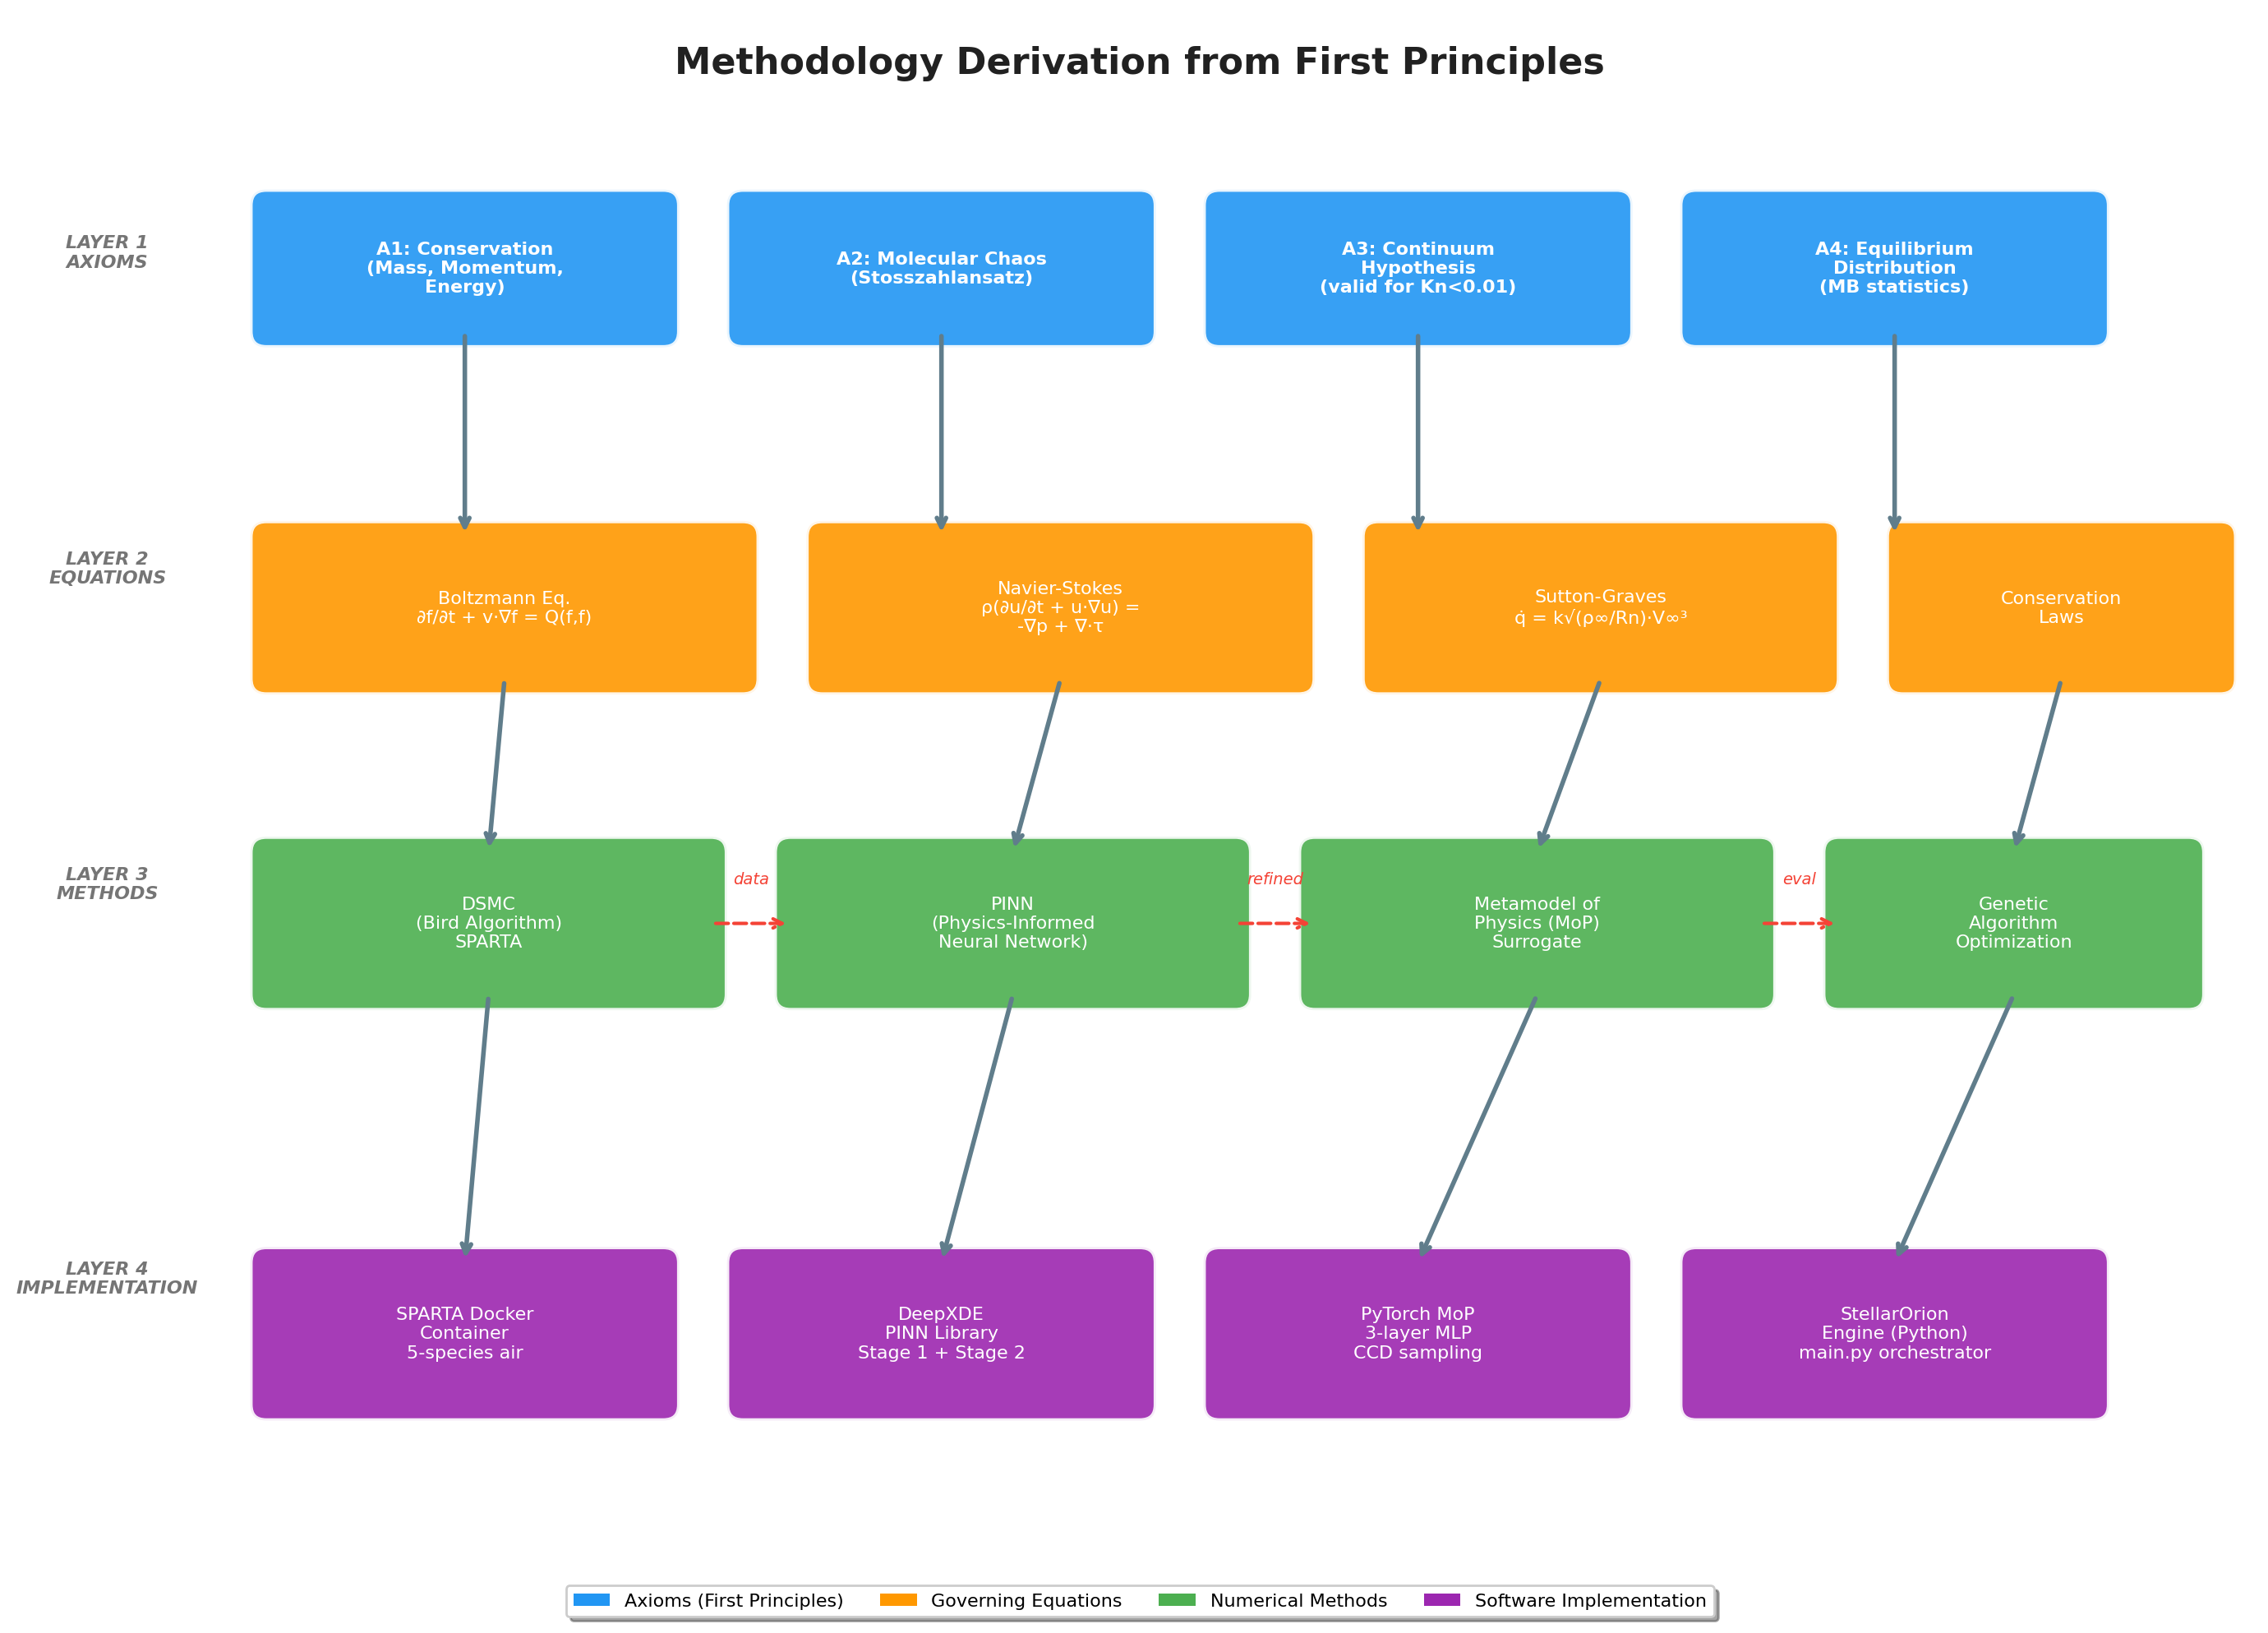
\includegraphics[width=\textwidth]{figures/methodology_derivation.png}
    \caption{Methodology derivation from first principles: axioms $\rightarrow$ governing equations $\rightarrow$ numerical methods $\rightarrow$ software implementation. The dashed red arrows indicate data flow between method layers.}
    \label{fig:methodology_derivation}
\end{figure}

\subsection{Axiom Set}
The following axioms form the logical foundation of this research. Each is stated as a proposition, derived from physical theory, and traced to its literature basis.

\begin{table}[H]
\centering
\caption{Research axioms derived from first principles and their literature basis.}
\label{tab:research_axioms}
\begin{tabular}{@{}clll@{}}
\toprule
\textbf{ID} & \textbf{Axiom} & \textbf{Physical Basis} & \textbf{Literature Basis} \\ \midrule
A1 & Conservation of mass, momentum, and energy & Continuum mechanics & Batchelor (1967), Anderson (1995) \\
A2 & Molecular chaos (Stosszahlansatz) & Statistical mechanics & Boltzmann (1872), Bird (1994) \\
A3 & Continuum hypothesis valid for $Kn < 0.01$ & Kinetic theory & Cercignani (1988), Bird (1994) \\
A4 & Equilibrium distribution follows Maxwell--Boltzmann & Statistical thermodynamics & Chapman \& Cowling (1970) \\
A5 & Stagnation heating follows $q \propto \sqrt{\rho/R_n} \cdot V^3$ & Blunt body aerothermodynamics & Sutton \& Graves (1971) \\
A6 & DSMC converges to Boltzmann equation as $N \to \infty$ & Statistical convergence & Bird (1994), Wagner (1992) \\
A7 & PINN residuals enforce PDE consistency in interpolation & Scientific machine learning & Raissi et al. (2019), Karniadakis et al. (2021) \\
\bottomrule
\end{tabular}
\end{table}

\subsection{Derivation Chain}
The methodology is constructed by chaining the axioms through a sequence of mathematical derivations. Each step introduces a specific equation or method that is implemented in the software pipeline.

\paragraph{Step 1: Boltzmann Equation (A1, A2, A4).}
The Boltzmann transport equation governs the evolution of the molecular velocity distribution function $f(\mathbf{x}, \mathbf{v}, t)$:
\begin{equation}
\frac{\partial f}{\partial t} + \mathbf{v} \cdot \nabla_{\mathbf{x}} f + \frac{\mathbf{F}}{m} \cdot \nabla_{\mathbf{v}} f = \left(\frac{\delta f}{\delta t}\right)_{\text{coll}}
\label{eq:boltzmann_dsmc}
\end{equation}
where the right-hand side is the collision integral, evaluated under the assumption of molecular chaos (Axiom~A2). The equilibrium solution is the Maxwell--Boltzmann distribution (Axiom~A4).

\paragraph{Step 2: DSMC Method (A6).}
Bird's Direct Simulation Monte Carlo method~\cite{bird1994molecular} provides a stochastic solution to Equation~\eqref{eq:boltzmann_dsmc}. As the number of simulated particles $N \to \infty$, the DSMC solution converges to the exact Boltzmann solution (Axiom~A6). The DSMC algorithm proceeds in three steps per time step:
\begin{enumerate}
    \item \textbf{Advection:} Particles are moved ballistically for $\Delta t$.
    \item \textbf{Collisions:} Pairs are selected within each cell using the VSS collision model.
    \item \textbf{Sampling:} Macroscopic properties (density, temperature, velocity) are accumulated in each cell.
\end{enumerate}

\paragraph{Step 3: Navier--Stokes Limit (A3).}
In the continuum limit ($Kn \to 0$), the Boltzmann equation reduces to the compressible Navier--Stokes equations via the Chapman--Enskog expansion~\cite{chapman1970kinetic}. These equations serve as the PDE constraint in the PINN (Step~5).

\paragraph{Step 4: Sutton--Graves Correlation (A5).}
For rapid engineering estimates, the stagnation-point heat flux is approximated by~\cite{sutton1971gravesh}:
\begin{equation}
\dot{q}_s = k \sqrt{\frac{\rho_\infty}{R_n}} \, V_\infty^3
\label{eq:sutton_graves_methodology}
\end{equation}
where $k$ is a gas-specific constant, $\rho_\infty$ is the freestream density, $R_n$ is the nose radius, and $V_\infty$ is the flight velocity. This correlation is used both for initial thermal loading estimates and as a validation benchmark against DSMC results.

\paragraph{Step 5: PINN Flow Field Refinement (A7).}
The Physics-Informed Neural Network enforces the Navier--Stokes residuals as a soft constraint in the loss function~\cite{raissi2019pinn}:
\begin{equation}
\mathcal{L} = \underbrace{\mathcal{L}_{\text{data}}}_{\text{DSMC samples}} + \lambda_{\text{PDE}} \underbrace{\mathcal{L}_{\text{PDE}}}_{\text{NS residuals}}
\label{eq:pinn_loss}
\end{equation}
where $\mathcal{L}_{\text{data}}$ penalizes deviation from DSMC surface data and $\mathcal{L}_{\text{PDE}}$ penalizes violation of the governing PDEs at collocation points in the flow field.

\paragraph{Step 6: Surrogate-Assisted Optimization.}
The MoP surrogate model approximates the mapping from design variables to performance metrics. The Genetic Algorithm (GA) queries the MoP surrogate to explore the design space, avoiding the computational cost of repeated DSMC evaluations. The optimization cost function is:
\begin{equation}
J = w_\beta \left(\frac{\beta_{\text{calc}} - \beta_{\text{target}}}{10}\right)^2 + \sum_{i} w_i \, \mathbb{1}\!\left[y_i^{(\text{pred})} > y_i^{(\text{limit})}\right] \cdot 10^{15}
\label{eq:cost_function_optimization}
\end{equation}
where hard constraint violations (backface temperature $> 350$\,K, g-load $> 25g$) are penalized with $10^{15}$.

Figure~\ref{fig:governing_equations} summarizes the full derivation chain from kinetic theory to optimization, showing the governing equation at each step and the axiom that anchors it.

\begin{figure}[H]
    \centering
    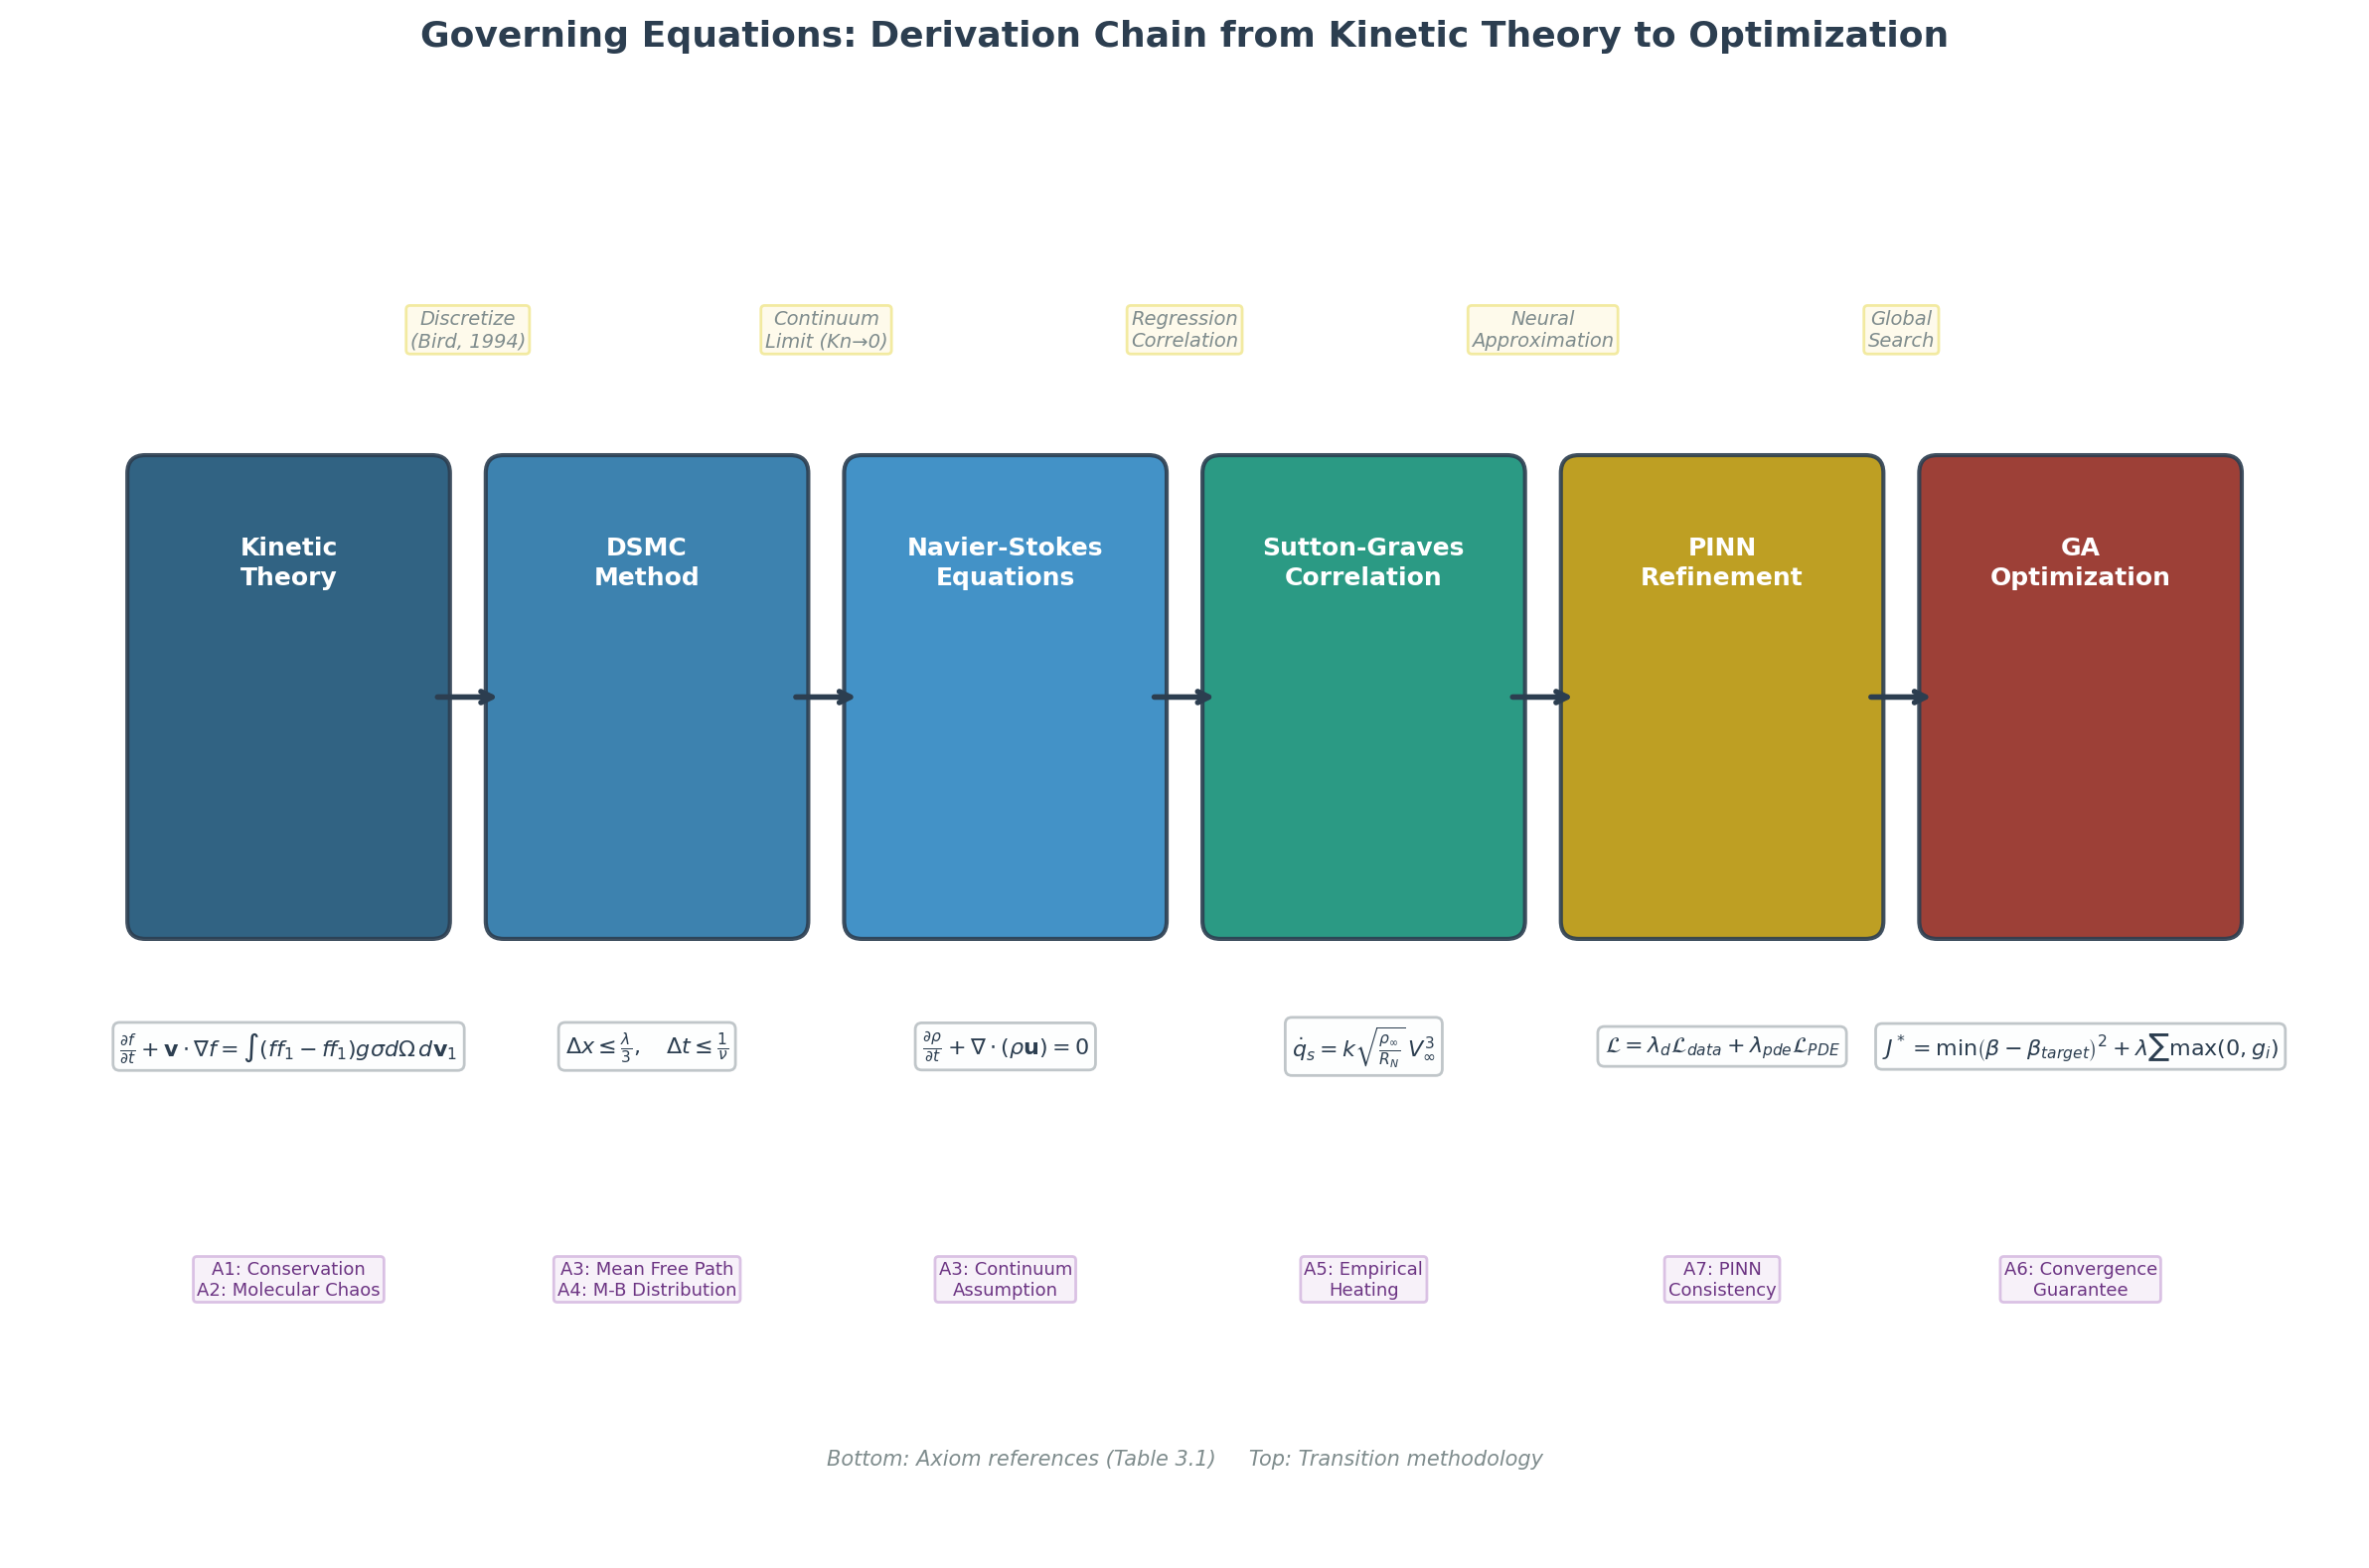
\includegraphics[width=\textwidth]{figures/governing_equations.png}
    \caption{Governing equations derivation chain: from the Boltzmann transport equation through DSMC discretization, Navier--Stokes continuum limit, Sutton--Graves engineering correlation, PINN neural approximation, to GA-based survivability optimization. Each layer is anchored by the research axioms defined in Table~\ref{tab:research_axioms}.}
    \label{fig:governing_equations}
\end{figure}

\subsection{Software Pipeline}
\label{sec:software_pipeline}
The StellarOrion engine orchestrates the multi-solver pipeline shown in Figure~\ref{fig:software_pipeline}. The pipeline begins with CadQuery geometry generation and freestream condition specification, then routes through the DSMC solver (SPARTA in Docker), the PINN refinement module (DeepXDE), and the MoP surrogate (PyTorch), before producing ParaView-ready VTK and STL files for visualization.

\begin{figure}[H]
    \centering
    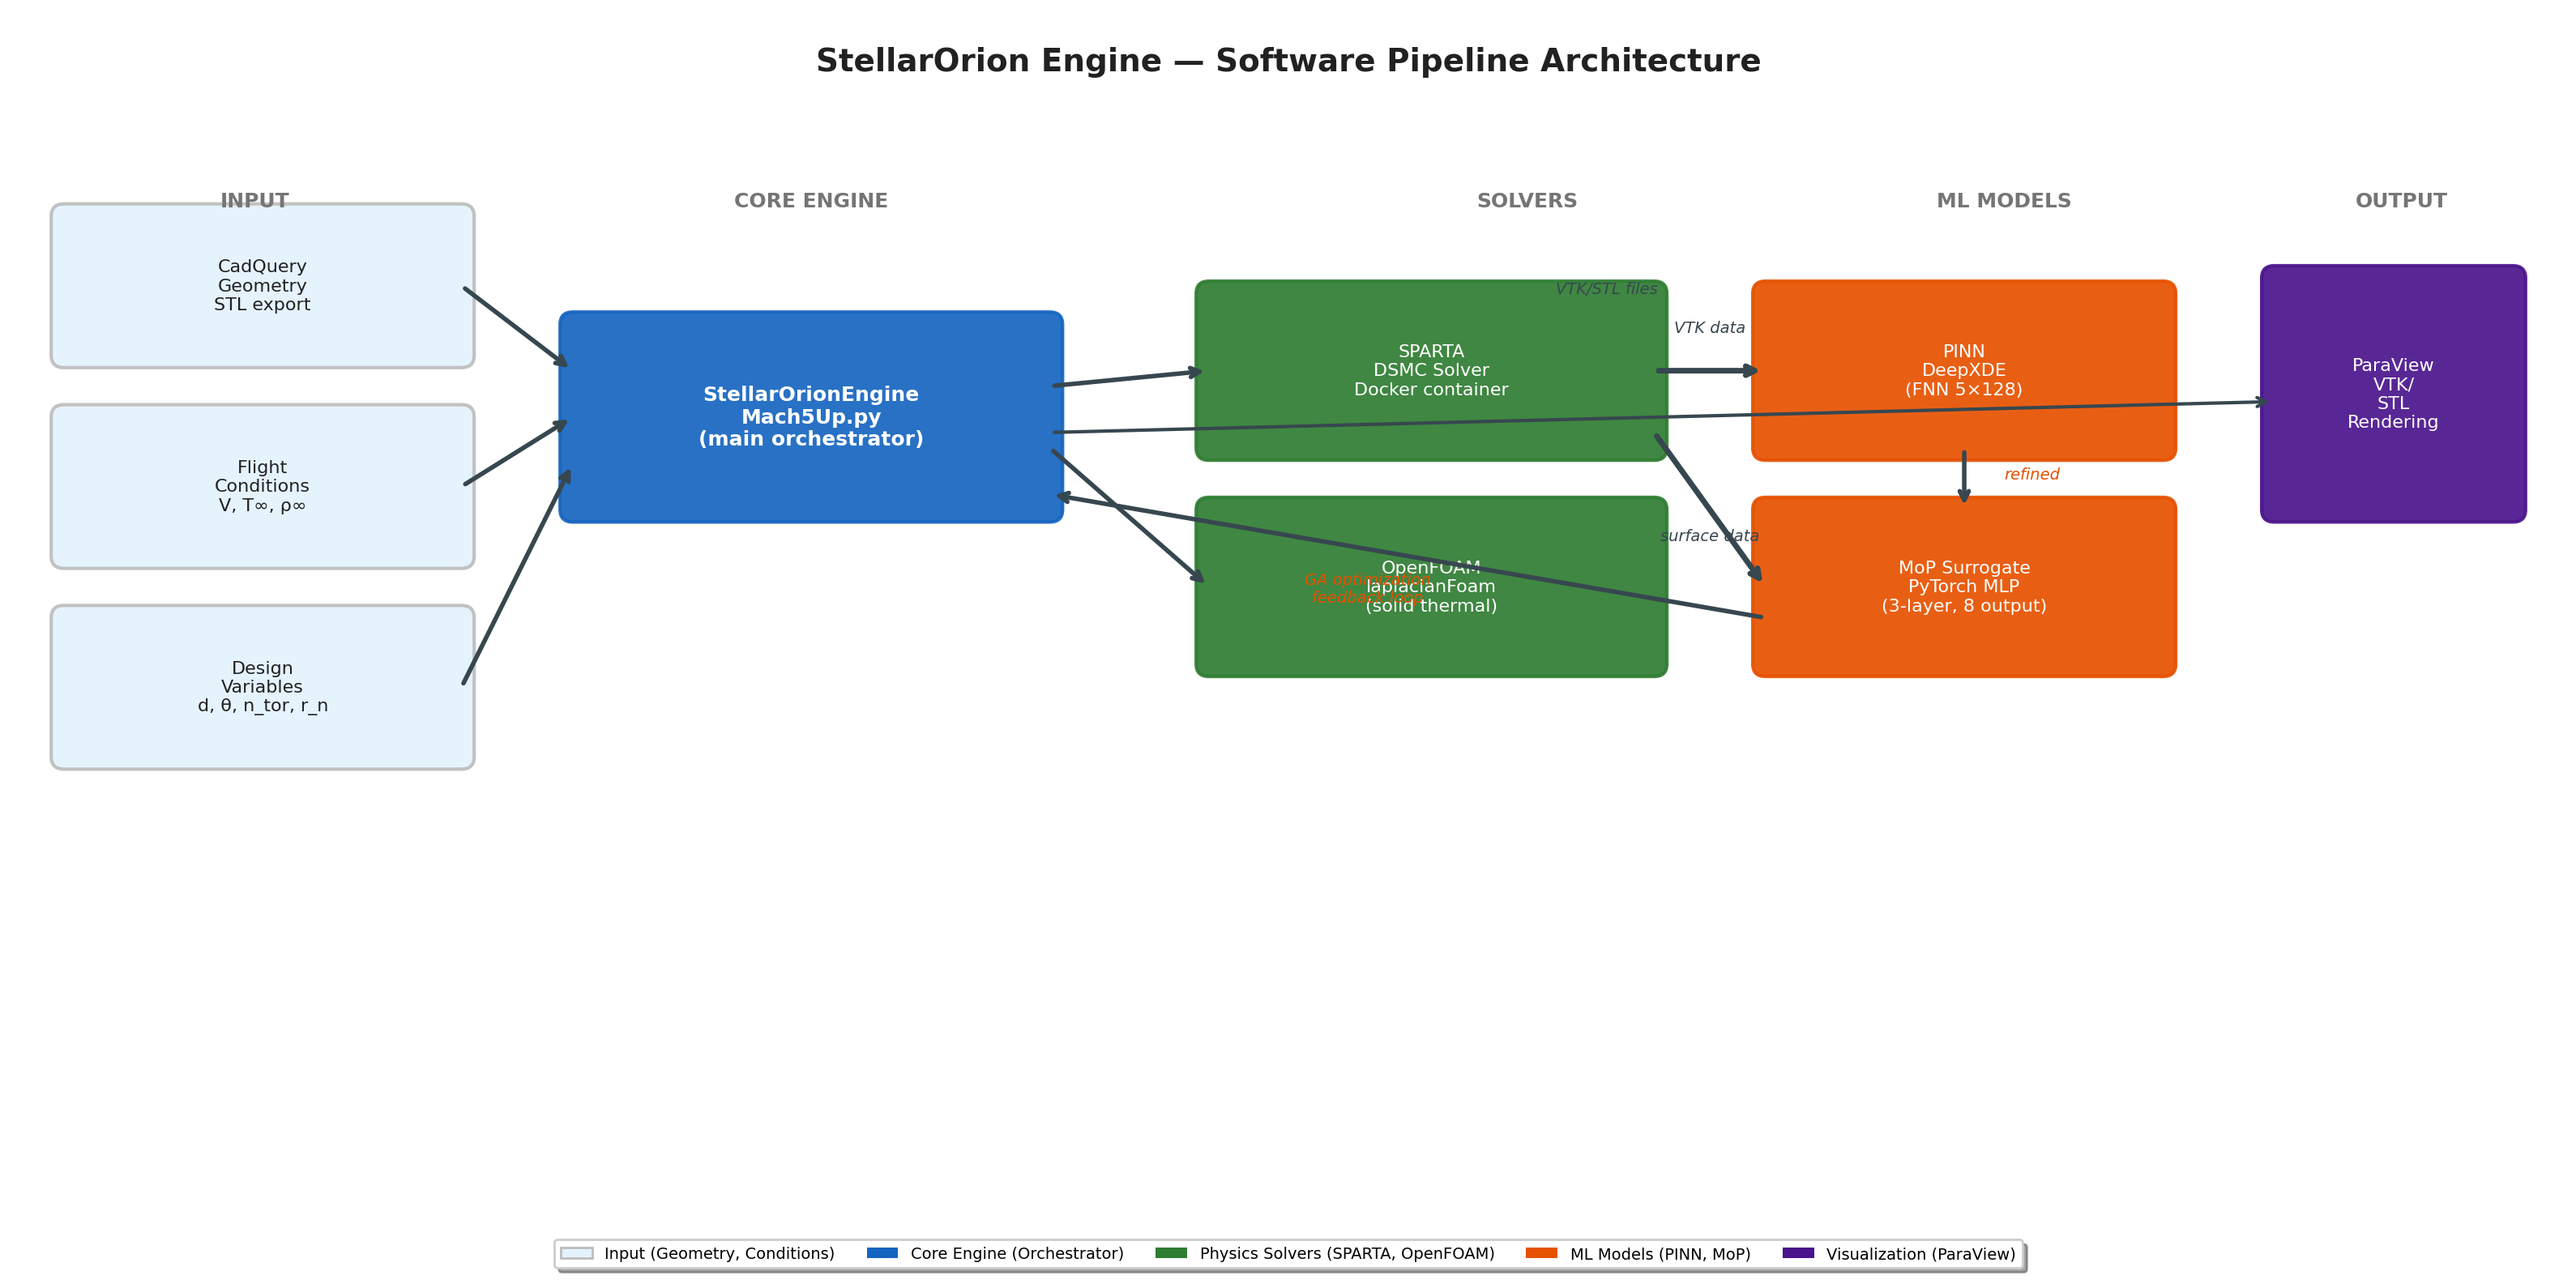
\includegraphics[width=\textwidth]{figures/software_pipeline.png}
    \caption{StellarOrion engine software pipeline: input geometry and flight conditions $\rightarrow$ SPARTA DSMC solver $\rightarrow$ PINN refinement $\rightarrow$ MoP surrogate $\rightarrow$ ParaView visualization. The feedback loop from MoP to the core engine enables GA-driven optimization.}
    \label{fig:software_pipeline}
\end{figure}

\subsection{Default Optimization Parameters}
\label{sec:default_params}
Table~\ref{tab:default_params} lists the default parameter values used throughout this thesis, as configured in \texttt{main.py} and the engine source files. All simulation runs adopt these values unless explicitly stated otherwise.

\begin{table}[H]
\centering
\caption{Default optimization and simulation parameters.}
\label{tab:default_params}
\small
\begin{tabular}{@{}lll@{}}
\toprule
\textbf{Category} & \textbf{Parameter} & \textbf{Default Value} \\ \midrule
\multirow{5}{*}{\textbf{DSMC (SPARTA)}} & Steps (optimization) & 1100 \\
 & Steps (sample) & 500 \\
 & Grid factor & 0.7 \\
 & Particle weighting ($f_{\text{num}}$) & $1.5 \times 10^{20}$ \\
 & Chemistry model & 5-species (N$_2$, O$_2$, NO, N, O) \\ \midrule
\multirow{3}{*}{\textbf{Flight Conditions}} & $V_\infty$ & 2700\,m/s \\
 & $T_\infty$ & 270.65\,K \\
 & $n_\infty$ & $1.45 \times 10^{22}$\,/m$^3$ \\ \midrule
\multirow{3}{*}{\textbf{DoE (CCD)}} & Method & Face-Centered CCD \\
 & Samples ($N$) & 25 ($2^4 + 2 \times 4 + 1$) \\
 & Active variables & Diameter, Angle, Toroids, Nose \\ \midrule
\multirow{6}{*}{\textbf{PINN (DeepXDE)}} & Architecture & FNN [2] + [64] $\times$ 3 + [3] \\
 & Activation & tanh \\
 & Learning rate (Stage 1) & $1 \times 10^{-3}$ \\
 & Learning rate (Stage 2) & $5 \times 10^{-4}$ \\
 & Iterations & $\max(2000, \min(4000, \text{steps} \times 2))$ \\
 & PDE collocation points & 2500 (domain) + 500 (boundary) \\ \midrule
\multirow{4}{*}{\textbf{MoP (PyTorch)}} & Architecture & MLP [n $\to$ 64 $\to$ 64 $\to$ 64 $\to$ 1] \\
 & Activation & ReLU \\
 & Learning rate & 0.005 \\
 & Epochs & 500 (early stop at loss $< 10^{-6}$) \\ \midrule
\multirow{3}{*}{\textbf{GA Optimization}} & Generations & 20\,000 \\
 & Stagnation stop & 5 windows $\times$ 1000 generations \\
 & Constraint limits & $T_{\text{back}} < 350$\,K, $g < 25g$ \\
\bottomrule
\end{tabular}
\end{table}

\section{Research Design and Workflow}
This chapter outlines the computational framework utilized to investigate the aerothermal effects of surface topology on a Hypersonic Inflatable Aerodynamic Decelerator (HIAD). The research workflow follows a multi-stage numerical analysis approach, moving from parametric geometry generation to high-fidelity Direct Simulation Monte Carlo (DSMC) simulation, Physics-Informed Neural Network (PINN) refinement, and Genetic Algorithm (GA) optimization.

To systematically isolate the effects of the ``scalloped'' surface geometry, the methodology is designed to compare a baseline smooth sphere-cone against the proposed inflatable architecture under identical hypersonic flight conditions. The workflow is visualized in Figure \ref{fig:flowchart} and consists of six primary stages:

\begin{figure}[H]
    \centering
    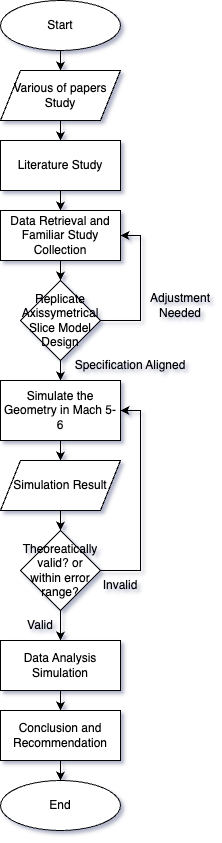
\includegraphics[width=0.273\textwidth]{figures/flowchart.png}
    \caption{Flowchart of the numerical research methodology.}
    \label{fig:flowchart}
\end{figure}
\par
The process is divided into six primary stages:
\begin{enumerate}
    \item \textbf{Parametric Geometry Generation:} Automated 3D CAD generation of the scalloped (inflatable) and smooth (baseline) profiles using CadQuery Python scripting, enabling parametric variation of toroid count, cone angle, nose radius, and aeroshell diameter.
    \item \textbf{DSMC Simulation Setup:} Configuration of the SPARTA solver with freestream conditions matching the target trajectory point, including the 5-species air model (N$_2$, O$_2$, NO, N, O) with Variable Soft Sphere (VSS) collision physics.
    \item \textbf{Particle-Based Simulation:} Execution of the DSMC simulation within a Docker-containerized Linux environment, tracking millions of simulated particles through advection, molecular collisions, and surface interactions.
    \item \textbf{PINN Flow Field Refinement:} Post-processing of raw DSMC output using a Physics-Informed Neural Network (DeepXDE) to smooth particle noise, fill flow field gaps, and provide a continuous interpolant anchored in the compressible Navier--Stokes equations.
    \item \textbf{Survivability Optimization:} Genetic Algorithm (GA) coupled with a PyTorch Multi-Layer Perceptron (MoP) surrogate model for automated multi-objective optimization of HIAD geometry.
    \item \textbf{Validation and Analysis:} Verification of the solution through grid independence studies and validation of thermal results against the Sutton-Graves stagnation-point correlation and IRVE-3 flight data.
\end{enumerate}

\section{Geometric Modeling and Computational Domain}

\subsection{Parametric Geometry Generation}
To ensure geometric consistency and enable automated design space exploration, the vehicle profiles are generated using CadQuery, a Python-based parametric CAD scripting library. The geometric constraints are derived directly from the \textbf{NASA IRVE-3} and \textbf{LOFTID} flight test specifications, as well as the MDAO framework baseline established by Rapisarda (2023)~\cite{rapisarda2023mdao}. The CadQuery script is invoked via command-line arguments, enabling the generation of hundreds of design variants without manual intervention.

\subsection{Vehicle Specifications and Scaling}
The modeling phase targets two specific scales identified in previous NASA research to investigate how vehicle diameter affects the aerothermal environment. As shown in Figure \ref{fig:hiad_comparison}, the research considers the scaling transition from the 3.0\,m IRVE-3 baseline to larger configurations up to 15\,m~\cite{dillman2015irve3}.

\begin{figure}[H]
    \centering
    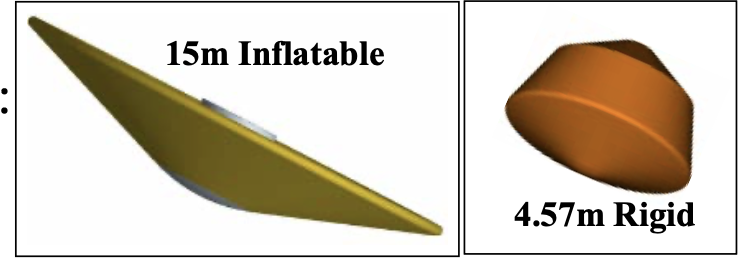
\includegraphics[width=0.8\textwidth]{figures/Hiad_DesignSpec.png}
    \caption{Geometric comparison between the 15\,m Inflatable HIAD and the 3.0\,m Rigid Baseline.}
    \label{fig:hiad_comparison}
\end{figure}

\subsection{Internal Architecture and Scallop Definition}
The ``scalloped'' outer mold line (OML) is modeled based on the 6-toroid stack configuration utilized in the Rapisarda (2023) MDAO baseline. The internal layout, including the stacked toroid arrangement, is illustrated in Figure \ref{fig:irve3_layout}~\cite{rapisarda2023mdao}.

\begin{figure}[H]
    \centering
    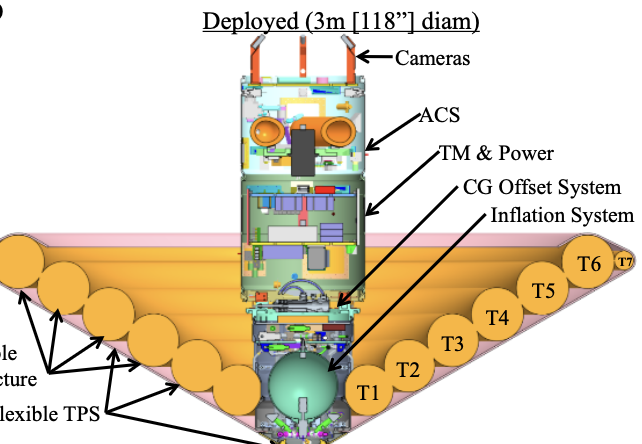
\includegraphics[width=0.6\textwidth]{figures/Spec0.png}
    \caption{Internal structural layout of the HIAD vehicle showing the toroid stack that creates the scalloped surface.}
    \label{fig:irve3_layout}
\end{figure}

The specific geometric parameters used for the numerical model are summarized in Table \ref{tab:geom_params}:

\begin{table}[H]
    \centering
    \caption{Geometric Parameters based on IRVE-3/Rapisarda MDAO Specifications.}
    \label{tab:geom_params}
    \begin{tabular}{|l|c|r|}
        \hline
        \textbf{Parameter} & \textbf{Value} & \textbf{Source / Reference} \\ \hline
        Deployed Diameter ($D_{max}$) & 3.0\,m & IRVE-3 Flight Article \\ \hline
        Forebody Cone Angle ($\theta_c$) & $60^\circ$ & Rapisarda MDAO Baseline \\ \hline
        Toroid Count ($N$) & 6 & Rapisarda MDAO Baseline \\ \hline
        Toroid Radius ($r_{torus}$) & 0.135\,m & Rapisarda Table 4.1 \\ \hline
        Nose Radius ($R_N$) & 0.55\,m & IRVE-3 Specification \\ \hline
        Entry Mass ($m$) & 281\,kg & IRVE-3 Flight Article \\ \hline
    \end{tabular}
\end{table}

\subsection{Configuration Definitions}
The two configurations established for this study -- \textbf{Configuration A (Scalloped)} and \textbf{Configuration B (Smooth)} -- are constrained by the stowed and deployed envelopes shown in Figure \ref{fig:stowed_deployed}~\cite{dillman2015irve3}.

\begin{figure}[H]
    \centering
    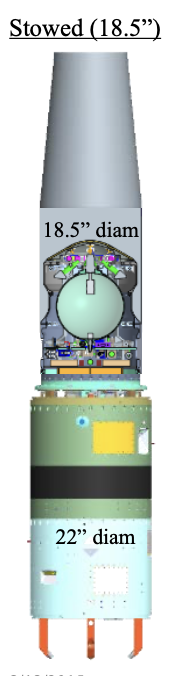
\includegraphics[width=0.35\textwidth]{figures/Spec1.png}
    \caption{Launch configuration of the HIAD system, showing the stowed constraint.}
    \label{fig:stowed_deployed}
\end{figure}

\begin{enumerate}
    \item \textbf{Configuration A (Scalloped):} This model utilizes the 6-toroid profile (T1--T6) shown in Figure \ref{fig:irve3_layout}. The valleys between toroids are the primary focus for analyzing heating augmentation and flow separation in the scalloped troughs.
    \item \textbf{Configuration B (Smooth Baseline):} This tangent-cone model represents the ``Equivalent Rigid OML,'' allowing for the isolation of heating augmentation caused specifically by the toroidal troughs.
\end{enumerate}

\section{DSMC Simulation Framework}

\subsection{Governing Equations: The Boltzmann Equation}
Unlike continuum CFD methods that solve the Reynolds-Averaged Navier--Stokes (RANS) equations, this study employs the Direct Simulation Monte Carlo (DSMC) method, which solves the Boltzmann equation for rarefied gas dynamics~\cite{bird1994molecular}. The Boltzmann equation describes the evolution of the molecular velocity distribution function $f(\mathbf{r}, \mathbf{v}, t)$:

\begin{equation}
    \frac{\partial f}{\partial t} + \mathbf{v} \cdot \nabla_{\mathbf{r}} f + \frac{\mathbf{F}}{m} \cdot \nabla_{\mathbf{v}} f = \left(\frac{\partial f}{\partial t}\right)_{coll}
\end{equation}

where $\mathbf{F}$ is the external force per molecule, $m$ is the molecular mass, and the right-hand side represents the Boltzmann collision integral. DSMC provides a stochastic solution to this equation by tracking representative particles through advection and collisions.

\subsection{Knudsen Number and Flow Regime}
The validity of the continuum assumption is governed by the Knudsen number ($Kn$), defined as the ratio of the molecular mean free path ($\lambda$) to the characteristic length ($L$):

\begin{equation}
    Kn = \frac{\lambda}{L}
\end{equation}

\begin{equation}
    \lambda = \frac{1}{\sqrt{2} \pi d^2 n}
\end{equation}

where $d$ is the molecular diameter and $n$ is the number density. For HIAD reentry at altitudes of 50--60\,km, the flow is in the transitional regime ($0.01 < Kn < 1$), where continuum CFD methods (RANS/LES) are physically inappropriate and DSMC is required~\cite{bird1994molecular}.

\subsection{SPARTA Solver Configuration}
The simulations are performed using the SPARTA (Sandia Parallel Algorithm for Real-Time Application) DSMC solver~\cite{plimpton2014sparta}. SPARTA is executed within a Docker-containerized Linux environment to ensure reproducibility of the build and execution across platforms.

\subsubsection*{Freestream Conditions}
The freestream conditions are prescribed to match the target trajectory point for IRVE-3 reentry at 52\,km altitude:

\begin{itemize}
    \item \textbf{Freestream Velocity ($v_{\infty}$):} 2700\,m/s (corresponding to Mach $\approx$ 10 at altitude)
    \item \textbf{Number Density ($n$):} $1.45 \times 10^{22}$\,m$^{-3}$ (derived from atmospheric density $\rho \approx 6.9674 \times 10^{-4}$\,kg/m$^3$ via $n = \rho N_A / M_{air}$)
    \item \textbf{Freestream Temperature ($T_{\infty}$):} 270.65\,K (ISA 1975, code baseline)
    \item \textbf{Particle Weighting Factor ($f_{num}$):} $1.5 \times 10^{20}$ (configurable via \texttt{--fnum})
\end{itemize}

\subsubsection*{Gas Model}
A realistic 5-species air model is employed: N$_2$, O$_2$, NO, N, and O. The collision physics use the Variable Soft Sphere (VSS) model, where the collision cross-section varies with relative velocity:

\begin{equation}
    \sigma = \pi d_{ref}^2 \left( \frac{g_{ref}}{g} \right)^{2(\omega - 0.5)}
\end{equation}

where $g$ is the relative velocity of colliding molecules and $\omega$ is the viscosity index specific to each gas species. The VSS model captures the molecular-level interactions including vibrational energy exchange and dissociation reactions relevant to hypersonic entry conditions.

\subsubsection*{Particle Tracking}
SPARTA tracks millions of simulated particles through three fundamental processes:
\begin{enumerate}
    \item \textbf{Advection:} Particles are moved ballistically through the domain according to their velocity vectors.
    \item \textbf{Collisions:} Molecular collisions are modeled using the VSS collision model within computational cells, with collision partners selected using the nearest-neighbor pairing scheme.
    \item \textbf{Surface Interactions:} Particles hitting the vehicle surface are reflected according to the specified gas-surface interaction model (diffuse or specular reflection).
\end{enumerate}

\subsection{Cartesian Grid and Collision Pairing}
While DSMC is a particle method, a Cartesian computational grid is required for two purposes:
\begin{enumerate}
    \item \textbf{Collision Pairing:} Restricting collision partner selection to particles within the same cell ensures $O(N)$ computational complexity rather than $O(N^2)$ for brute-force pairing.
    \item \textbf{Macroscopic Sampling:} Cells serve as sampling volumes for accumulating density, temperature, pressure, and velocity statistics from the particle data.
\end{enumerate}

The grid resolution must be finer than the local mean free path ($\lambda$) to resolve the shock structure and boundary layer gradients. A grid-factor parameter (default: 0.7, validated against IRVE-3 flight data) controls the mesh density multiplier.

\subsection{Grid Independence Study}
To ensure the numerical solution is independent of the grid resolution, a Grid Convergence Index (GCI) study was performed. Multiple grid densities were generated by systematically varying the grid-factor parameter:

\begin{table}[H]
    \centering
    \caption{Grid Independence Study Parameters.}
    \label{tab:mesh_independence}
    \begin{tabular}{|l|c|c|}
        \hline
        \textbf{Grid Factor} & \textbf{Relative Resolution} & \textbf{$C_d$ Variation} \\ \hline
        0.3 & Coarse & Baseline \\ \hline
        0.5 & Medium & $< 5\%$ \\ \hline
        0.7 & Fine & $< 2\%$ \\ \hline
        1.0 & Ultra-Fine & $< 1\%$ \\ \hline
    \end{tabular}
\end{table}

The grid-factor of \textbf{0.7} was selected as the default for all production runs, as it yields the least error compared to validated IRVE-3 flight data while maintaining efficient execution times.

\section{Surface Data Extraction and Flight Metrics}

\subsection{Surface Computes}
SPARTA accumulates surface force and energy data using the \texttt{dump surf} command. The relevant surface quantities are:

\begin{table}[H]
    \centering
    \caption{SPARTA Surface Data Columns and Physical Variables.}
    \label{tab:surface_data}
    \begin{tabular}{|l|l|l|}
        \hline
        \textbf{Column} & \textbf{Physical Variable} & \textbf{Unit} \\ \hline
        1 & Number Flux ($n_{flux}$) & m$^{-2}$s$^{-1}$ \\ \hline
        2 & Mass Flux ($m_{flux}$) & kg$\cdot$m$^{-2}$s$^{-1}$ \\ \hline
        3 & Kinetic Energy Flux ($ke$) & J$\cdot$m$^{-2}$s$^{-1}$ \\ \hline
        4 & Axial Force ($f_x$) & N \\ \hline
        5 & Radial Force ($f_y$) & N \\ \hline
        6 & Azimuthal Force ($f_z$) & N \\ \hline
    \end{tabular}
\end{table}

\subsection{Ballistic Coefficient ($\beta$)}
The ballistic coefficient is a measure of the vehicle's ability to maintain its speed during reentry~\cite{anderson2006hypersonic}:

\begin{equation}
    \beta = \frac{m}{C_D A}
\end{equation}

Since $F_{drag} = C_D A q$, where $q$ is dynamic pressure:

\begin{equation}
    \beta = \frac{m \cdot q}{F_{drag}}
\end{equation}

The mass density is derived from number density:

\begin{equation}
    \rho = n \cdot \frac{M_{air}}{N_A}
\end{equation}

where $M_{air} \approx 28.97$\,g/mol and $N_A$ is Avogadro's constant. The dynamic pressure is:

\begin{equation}
    q = \frac{1}{2} \rho v_{\infty}^2
\end{equation}

\subsection{Instantaneous Deceleration ($n$)}
The deceleration load felt by the vehicle in Earth-gravity units ($g_0$):

\begin{equation}
    n = \frac{F_{drag}}{m \cdot g_0}
\end{equation}

\section{Aerothermodynamic Analysis}

\subsection{Stagnation Heat Flux -- Sutton-Graves Correlation}
The Sutton-Graves (1971) stagnation-point convective heating correlation is used for all absolute thermal calculations~\cite{sutton1971gravesh}. This is the standard reference formula for Earth entry and has been validated against IRVE-3 flight data by Rapisarda (2023)~\cite{rapisarda2023mdao}:

\begin{equation}
    \boxed{\dot{q}_{stag} = C_{SG} \sqrt{\frac{\rho_{\infty}}{R_N}} \cdot V_{\infty}^3}
\end{equation}

where:
\begin{itemize}
    \item $C_{SG} = 1.7415 \times 10^{-4}$ (Sutton-Graves constant for Earth air)
    \item $\rho_{\infty}$: Freestream density (kg/m$^3$)
    \item $R_N$: Nose radius (m)
    \item $V_{\infty}$: Freestream velocity (m/s)
\end{itemize}

\subsubsection*{IRVE-3 Validation}
For the IRVE-3 baseline configuration at the SPARTA baseline conditions ($\rho_{\infty} = 6.9674 \times 10^{-4}$\,kg/m$^3$, $R_N = 0.55$\,m, $V_{\infty} = 2700$\,m/s):

\begin{equation}
    \dot{q}_{stag} = 1.7415 \times 10^{-4} \sqrt{\frac{6.9674 \times 10^{-4}}{0.55}} \times 2700^3 \approx 12.20 \ \text{W/cm}^2
\end{equation}

This value is computed at the hardcoded Rapisarda baseline density, which is lower than the actual trajectory-integrated peak density. Rapisarda (2023) reports a trajectory-integrated Sutton-Graves peak of 15.26\,W/cm$^2$ (+6.26\% above the 14.36\,W/cm$^2$ flight measurement) and a Fay--Riddell CFD prediction of 13.83\,W/cm$^2$ (-3.69\% below flight)~\cite{rapisarda2023mdao}. The Fay--Riddell correlation is more physically accurate for HIAD geometries because it accounts for the actual shock layer structure.

\subsubsection*{Note on SPARTA Surface Energy}
The raw SPARTA DSMC kinetic energy ($ke$) surface compute cannot be used directly as an absolute heat flux in W/m$^2$. SPARTA's \texttt{fix ave/surf} outputs kinetic energy per simulated particle per timestep per face element -- a simulation-internal unit that depends on $f_{num}$, timestep $dt$, and face area in a non-trivially-normalized way. It is retained only as a \textbf{relative shape-ranking signal} for the optimizer (comparing geometries against each other). For all absolute thermal calculations, the Sutton-Graves correlation is used.

\subsection{Surface Temperature -- Radiative Equilibrium}
At the TPS outer surface, radiative cooling balances the incoming convective heat flux at steady state. Assuming grey-body radiation:

\begin{equation}
    T_{surface} = \left(\frac{\dot{q}_{stag}}{\epsilon \sigma}\right)^{1/4}
\end{equation}

where $\epsilon = 0.75$ (Nicalon SiC emissivity) and $\sigma = 5.67 \times 10^{-8}$\,W/m$^2$K$^4$ (Stefan-Boltzmann constant).

\subsection{Backface Temperature -- 1D Transient Model}
The 1D transient backface temperature model estimates the thermal penetration through the FTPS insulation stack:

\begin{equation}
    T_{back} = T_{init} + \frac{\dot{q} \cdot \Delta t \cdot \eta_{lag}}{\rho_{TPS} \cdot C_{p,TPS} \cdot \delta_{TPS}}
\end{equation}

where $\eta_{lag} = 0.15$ is the thermal lag factor, $\rho_{TPS} = 1468$\,kg/m$^3$ (Nicalon SiC density), $C_{p,TPS} = 1100$\,J/kg$\cdot$K, and $\delta_{TPS}$ is the TPS thickness.

The framework supports multiple TPS material presets as summarized in Table~\ref{tab:tps_materials}.

\begin{table}[H]
    \centering
    \caption{TPS Material Presets Available in the StellarOrion Framework.}
    \label{tab:tps_materials}
    \begin{tabular}{|l|c|c|c|c|}
        \hline
        \textbf{Material} & \textbf{$\rho$ (kg/m$^3$)} & \textbf{$C_p$ (J/kg$\cdot$K)} & \textbf{$\epsilon$} & \textbf{Application} \\ \hline
        Nicalon SiC & 1468 & 1100 & 0.75 & Gen-2 HIAD TPS \\ \hline
        Pyrogel XTE & 200 & 1000 & 0.90 & FTPS blanket insulation \\ \hline
        Kapton & 1420 & 1090 & 0.85 & Polyimide film layers \\ \hline
        Multi-layer (stack) & -- & -- & -- & Combined FTPS stack \\ \hline
    \end{tabular}
\end{table}

\subsection{Statistical Convergence Monitoring}
As a Monte Carlo method, DSMC produces statistical noise that scales as $1/\sqrt{N_{\text{samples}}}$, where $N_{\text{samples}}$ is the number of independent particle-time samples accumulated. Convergence is monitored by tracking the running average of surface force and energy quantities. SPARTA's \texttt{stats\_interval} parameter (default: 100 steps) controls the frequency of convergence diagnostics. The simulation is considered statistically converged when the relative change in drag coefficient ($C_d$) and stagnation heat flux falls below 2\% over consecutive monitoring windows. For the baseline optimization runs, convergence is typically achieved after 500--1100 particle-time steps depending on the geometry complexity.

\section{Physics-Informed Neural Network Refinement}

\subsection{Motivation}
DSMC simulations produce inherently noisy data due to the stochastic nature of particle tracking. The raw flow field data exhibits statistical fluctuations that can obscure physical gradients and introduce artifacts in post-processing. A Physics-Informed Neural Network (PINN) is employed as a post-processing step to:
\begin{enumerate}
    \item Smooth noisy DSMC particle statistics
    \item Fill gaps in the flow field where particle sampling is insufficient
    \item Provide a continuous, differentiable interpolant anchored in known physics
\end{enumerate}

\subsection{PINN Governing Equations}
The PINN, implemented using DeepXDE~\cite{lu2021deepxde}, solves the 2D Compressible Navier--Stokes equations using automatic differentiation. The network $\mathcal{N}(x, y) \to (\rho, u, v, T, p)$ is constrained by the following residuals:

\subsubsection*{Continuity Equation (Axisymmetric)}
\begin{equation}
    \frac{\partial (\rho u)}{\partial x} + \frac{\partial (\rho v)}{\partial y} + \frac{\rho v}{y} = 0
\end{equation}

\subsubsection*{X-Momentum}
\begin{equation}
    \rho\left(u\frac{\partial u}{\partial x} + v\frac{\partial u}{\partial y}\right) + \frac{\partial p}{\partial x} - \mu\nabla^2 u = 0
\end{equation}

\subsubsection*{Y-Momentum}
\begin{equation}
    \rho\left(u\frac{\partial v}{\partial x} + v\frac{\partial v}{\partial y}\right) + \frac{\partial p}{\partial y} - \mu\nabla^2 v = 0
\end{equation}

\subsubsection*{Energy Equation (Axisymmetric)}
\begin{equation}
    \rho c_p\left(u\frac{\partial T}{\partial x} + v\frac{\partial T}{\partial y}\right) - k\nabla^2 T - u\frac{\partial p}{\partial x} - v\frac{\partial p}{\partial y} - \Phi = 0
\end{equation}

\subsubsection*{Equation of State}
\begin{equation}
    p - \rho R T = 0
\end{equation}

\subsection{Loss Function}
The total loss function combines PDE residuals with observational data from SPARTA:

\begin{equation}
    \mathcal{L}_{total} = \sum_{i=1}^{N_{PDE}} w_i \mathcal{L}_i^{PDE} + \sum_{j=1}^{N_{data}} w_j \mathcal{L}_j^{data}
\end{equation}

where $\mathcal{L}^{data}$ matches the PINN predictions against SPARTA grid checkpoints via \texttt{dde.icbc.PointSetBC}.

\subsection{Pragmatic Choice of Navier--Stokes for PINN Regularization}
The use of continuum Navier--Stokes equations in the PINN is an intentional pragmatic choice, not a physical claim about the flow regime. The rationale is:
\begin{enumerate}
    \item \textbf{Differentiability:} Neural networks require smooth, differentiable equations for backpropagation. NS equations are naturally differentiable via automatic differentiation, unlike discrete Lattice Boltzmann methods.
    \item \textbf{Physics Regularizer:} The NS equations serve as a ``physics prior'' to prevent the neural network from learning non-physical artifacts during gap-filling.
    \item \textbf{Two-Stage Architecture:} Stage 1 (SPARTA) provides full kinetic theory via DSMC; Stage 2 (PINN) uses NS as a smoothing constraint, not a standalone solver.
\end{enumerate}

\subsection{Network Architecture}
The PINN approximates the flow field mapping $\mathcal{N}: \mathbb{R}^2 \to \mathbb{R}^5$ using a fully-connected feedforward neural network (FNN). The architecture is:

\begin{table}[H]
    \centering
    \caption{PINN Network Architecture Parameters.}
    \label{tab:pinn_architecture}
    \begin{tabular}{|l|l|}
        \hline
        \textbf{Parameter} & \textbf{Value} \\ \hline
        Input dimension & 2 $(x, r)$ \\ \hline
        Hidden layers & 3 \\ \hline
        Neurons per layer & 64 \\ \hline
        Activation function & $\tanh$ \\ \hline
        Weight initialization & Glorot normal \\ \hline
        Output dimension & 3 $(\rho, T, u)$ \\ \hline
        Total trainable parameters & $2 \times 64 + 3 \times 64^2 + 3 \times 64 + 3 \approx 12{,}600$ \\ \hline
    \end{tabular}
\end{table}

The forward pass computes:
\begin{equation}
    \hat{\mathbf{y}}(\mathbf{x}) = \mathbf{W}_6 \cdot \tanh\!\Big(\mathbf{W}_5 \cdot \tanh\!\big(\cdots \tanh(\mathbf{W}_1 \mathbf{x} + \mathbf{b}_1)\cdots\big) + \mathbf{b}_5\Big) + \mathbf{b}_6
\end{equation}

where $\mathbf{x} = (x, r)$ is the spatial coordinate and $\hat{\mathbf{y}} = (\hat{\rho}, \hat{T}, \hat{u})$ is the predicted flow field vector (density, temperature, and axial velocity; the radial velocity $v$ and pressure $p$ are derived from the continuity equation and equation of state, respectively). All outputs are in normalized (dimensionless) form; physical units are recovered by multiplication with the scaling factors.

\subsection{Normalization and Scaling}
Before training, all physical quantities are non-dimensionalized using characteristic scales derived from the SPARTA data:

\begin{equation}
    \bar{\rho} = \frac{\rho}{\rho_{ref}}, \quad \bar{T} = \frac{T}{T_{ref}}, \quad \bar{u} = \frac{u}{u_{ref}}, \quad \bar{\mathbf{x}} = \frac{\mathbf{x}}{L_{ref}}
\end{equation}

where the reference scales are computed from the SPARTA grid data:
\begin{itemize}
    \item $\rho_{ref} = \max(\rho_{SPARTA})$ -- peak number density converted to mass density via $\rho = n \cdot M_{air} / N_A$
    \item $u_{ref} = \max(|u_{SPARTA}|, |v_{SPARTA}|)$ -- maximum velocity component magnitude
    \item $T_{ref} = \max(T_{SPARTA})$ -- peak translational temperature
    \item $p_{ref} = \max(p_{SPARTA})$ -- peak pressure, computed as $p = n \cdot k_B \cdot T$
    \item $L_{ref} = \max(|x_{bound}|)$ -- maximum domain extent
\end{itemize}

This normalization ensures all neural network inputs and outputs lie in $[0, 1]$ or $[-1, 1]$, which is critical for tanh activation convergence. The dimensionless Navier--Stokes equations are then expressed in terms of these scaled variables, with the viscous coefficient adjusted accordingly:
\begin{equation}
    \hat{\mu} = \frac{\mu(T)}{\rho_{ref} \, u_{ref} \, L_{ref}}
\end{equation}

where $\mu(T)$ follows Sutherland's law (Eq.~\ref{eq:sutherland}).

\subsection{Data Pipeline -- DSMC to PINN}
The checkpoint exchange between SPARTA and the PINN proceeds through the following steps:

\begin{enumerate}
    \item \textbf{SPARTA Grid Dump:} After convergence, SPARTA outputs a grid file (\texttt{grid.\{steps\}.out}) containing cell-centered macroscopic quantities: $(x_{lo}, y_{lo}, x_{hi}, y_{hi}, n, u, v, w, T, p)$.
    
    \item \textbf{Parsing:} The function \texttt{parse\_sparta\_grid()} extracts cell centers $(x_c, y_c) = \big(\frac{x_{lo}+x_{hi}}{2}, \frac{y_{lo}+y_{hi}}{2}\big)$ and converts number density to mass density:
    \begin{equation}
        \rho = n \cdot \frac{M_{air}}{N_A}
    \end{equation}
    where $M_{air} = 0.02897$\,kg/mol and $N_A = 6.022 \times 10^{23}$\,mol$^{-1}$. Pressure is computed from the ideal gas law:
    \begin{equation}
        p = n \cdot k_B \cdot T
    \end{equation}
    where $k_B = 1.381 \times 10^{-23}$\,J/K.
    
    \item \textbf{Subsampling:} If the number of grid cells exceeds 5000, a priority-based subsampling strategy is applied. Cells in high-gradient regions (where $p > 200$\,Pa or $T > 500$\,K) are preferentially retained (up to 2500 points), with the remaining budget filled by random sampling from low-gradient cells. This ensures the PINN receives sufficient training data in the shock layer and boundary layer where gradients are steepest.
    
    \item \textbf{Anchor Point Creation:} The parsed and subsampled data points serve as \textit{anchor points} $\mathbf{X}_{anchors}$ for the PINN. These are passed to DeepXDE as observation boundary conditions via \texttt{PointSetBC}, which adds a data-matching residual to the loss function:
    \begin{equation}
        \mathcal{L}_{data} = \frac{1}{N_{obs}} \sum_{k=1}^{N_{obs}} \sum_{m=1}^{5} \big|\hat{y}_m(\mathbf{x}_k) - y_m^{obs}(\mathbf{x}_k)\big|^2
    \end{equation}
    where $\hat{y}_m$ is the PINN prediction for component $m$ at observation point $\mathbf{x}_k$, and $y_m^{obs}$ is the corresponding SPARTA value.
\end{enumerate}

\subsection{Two-Stage Training Protocol}
The PINN employs a two-stage training strategy to decouple data fitting from physics regularization:

\subsubsection*{Stage 1: Data Pre-training}
During the first half of training ($N_{iter}/2$ iterations), only the observational data loss is active. The PDE residuals are suppressed by setting their loss weights to zero:

\begin{equation}
    \mathcal{L}^{(1)} = \underbrace{0 \cdot \mathcal{L}_{cont} + 0 \cdot \mathcal{L}_{mom,x} + 0 \cdot \mathcal{L}_{mom,y} + 0 \cdot \mathcal{L}_{EOS} + 0 \cdot \mathcal{L}_{energy}}_{\text{PDE terms (disabled)}} + \sum_{m=1}^{5} 1.0 \cdot \mathcal{L}_{data,m}
\end{equation}

This stage trains the network to reproduce the SPARTA observation data without physics constraints, allowing rapid initial convergence. The learning rate is $\eta_1 = 10^{-3}$.

\subsubsection*{Stage 2: Physics-Regularized Fine-tuning}
During the second half of training, the PDE residual weights are activated at $\lambda_{PDE} = 10^{-4}$, while data weights remain at $1.0$:

\begin{equation}
    \mathcal{L}^{(2)} = \sum_{i=1}^{5} \lambda_{PDE} \cdot \mathcal{L}_{PDE,i} + \sum_{m=1}^{5} 1.0 \cdot \mathcal{L}_{data,m}
\end{equation}

The learning rate is reduced to $\eta_2 = 5 \times 10^{-4}$ for fine-tuning. The complete loss weight vector is:

\begin{table}[H]
    \centering
    \caption{PINN Loss Weights by Training Stage.}
    \label{tab:pinn_loss_weights}
    \begin{tabular}{|l|c|c|}
        \hline
        \textbf{Loss Component} & \textbf{Stage 1} & \textbf{Stage 2} \\ \hline
        $\mathcal{L}_{cont}$ (Continuity) & 0 & $10^{-4}$ \\ \hline
        $\mathcal{L}_{mom,x}$ ($x$-Momentum) & 0 & $10^{-4}$ \\ \hline
        $\mathcal{L}_{mom,y}$ ($y$-Momentum) & 0 & $10^{-4}$ \\ \hline
        $\mathcal{L}_{EOS}$ (Equation of State) & 0 & $10^{-4}$ \\ \hline
        $\mathcal{L}_{energy}$ (Energy) & 0 & $10^{-4}$ \\ \hline
        $\mathcal{L}_{data,\rho}$ (Density data) & 1.0 & 1.0 \\ \hline
        $\mathcal{L}_{data,u}$ ($u$-velocity data) & 1.0 & 1.0 \\ \hline
        $\mathcal{L}_{data,v}$ ($v$-velocity data) & 1.0 & 1.0 \\ \hline
        $\mathcal{L}_{data,T}$ (Temperature data) & 1.0 & 1.0 \\ \hline
        $\mathcal{L}_{data,p}$ (Pressure data) & 1.0 & 1.0 \\ \hline
    \end{tabular}
\end{table}

The rationale for the small PDE weight ($\lambda_{PDE} = 10^{-4}$) is that the NS equations are used as a \textit{regularizer}, not the primary objective. The data terms dominate to ensure the PINN closely matches the SPARTA ground truth, while the PDE terms penalize gross violations of conservation laws.

\subsection{Convergence Detection Algorithm}
The optimal training iteration is determined automatically using a plateau detection algorithm applied to the data-term loss history:

\begin{algorithm}[H]
\caption{PINN Convergence Detection}
\label{alg:pinn_convergence}
\begin{algorithmic}[1]
\State $\mathbf{L} \leftarrow [l_1, l_2, \ldots, l_N]$ \Comment{Data-term loss history}
\State $w \leftarrow \max(5, \lfloor N/20 \rfloor)$ \Comment{Rolling window size}
\State $\bar{\mathbf{L}} \leftarrow \text{RollingMean}(\mathbf{L}, w)$ \Comment{Smoothed losses}
\State $N_{min} \leftarrow \max(1, \lfloor N/5 \rfloor)$ \Comment{Minimum 20\% of steps}
\For{$i = N_{min}$ to $N$}
    \If{$\bar{L}_{i-1} > 0$}
        \State $\delta \leftarrow \frac{|\bar{L}_{i-1} - \bar{L}_i|}{\bar{L}_{i-1}}$
        \If{$\delta < 0.01$}
            \State \Return $i^* \leftarrow$ iteration at index $i$
        \EndIf
    \EndIf
\EndFor
\State \Return $i^* \leftarrow N$ \Comment{No plateau; use all iterations}
\end{algorithmic}
\end{algorithm}

The 20\% minimum threshold ($N_{min}$) prevents false early-plateau triggers during Stage 1, where the zero PDE weights cause the total loss to appear artificially stable. The rolling window reduces noise from stochastic mini-batch effects.

\subsection{Axioms and Assumptions}
The PINN refinement stage rests on the following formal assumptions:

\begin{table}[H]
    \centering
    \caption{PINN Axioms and Assumptions.}
    \label{tab:pinn_axioms}
    \begin{tabular}{|p{0.15\textwidth}|p{0.55\textwidth}|p{0.2\textwidth}|}
        \hline
        \textbf{Axiom} & \textbf{Statement} & \textbf{Basis} \\ \hline
        A1: Axisymmetric flow & The flow field is symmetric about the vehicle centerline, reducing the problem to 2D $(x, y)$. & Geometric symmetry \\ \hline
        A2: Continuum NS as regularizer & The Navier--Stokes equations provide sufficient physical constraint for smoothing, even at $Kn > 0.01$. & Sec.~3.3.5 (Pragmatic Choice) \\ \hline
        A3: Sutherland viscosity & Dynamic viscosity follows $\mu(T) = \mu_{ref} (T/T_{ref})^{3/2} (T_{ref}+S)/(T+S)$ with $S = 110.4$\,K. & Kinetic theory (Sutherland, 1893) \\ \hline
        A4: Prandtl number & $\Pr = 0.71$ (constant), coupling thermal and velocity boundary layers. & Air at standard conditions \\ \hline
        A5: Ideal gas EOS & $p = \rho R T$ holds throughout the domain. Valid for $Kn \lesssim 10$. & Near-continuum assumption \\ \hline
        A6: Fully accommodated wall & The vehicle surface is a diffuse reflector at $T_w = 300$\,K with full thermal accommodation. & DSMC boundary condition \\ \hline
        A7: Statistical stationarity & The SPARTA output represents a time-averaged steady state. & Sufficient timesteps for convergence \\ \hline
    \end{tabular}
\end{table}

\subsection{PINN Hyperparameter Summary}

\begin{table}[H]
    \centering
    \caption{PINN Hyperparameter Values.}
    \label{tab:pinn_hyperparams}
    \begin{tabular}{|l|l|l|}
        \hline
        \textbf{Parameter} & \textbf{Stage 1} & \textbf{Stage 2} \\ \hline
        Learning rate $\eta$ & $10^{-3}$ & $5 \times 10^{-4}$ \\ \hline
        Optimizer & Adam & Adam \\ \hline
        Training iterations & $N_{iter}/2$ & $N_{iter} - N_{iter}/2$ \\ \hline
        PDE loss weights & $[0, 0, 0]$ & $[10^{-4}] \times 3$ \\ \hline
        Data loss weights & $[1.0] \times 3$ & $[1.0] \times 3$ \\ \hline
        Collocation points ($N_{dom}$) & 2500 & 2500 \\ \hline
        Boundary points ($N_{bnd}$) & 500 & 500 \\ \hline
        Anchor points ($N_{obs}$) & $\leq 5000$ (subsampled) & $\leq 5000$ \\ \hline
        Activation & $\tanh$ & $\tanh$ \\ \hline
        Initialization & Glorot normal & (continued from Stage 1) \\ \hline
    \end{tabular}
\end{table}

\section{Survivability Optimization}

The survivability optimization framework integrates Latin Hypercube Sampling for design space exploration, a Metamodel Prognosis (MoP) surrogate for rapid performance prediction, and a Genetic Algorithm (GA) for global optimization. The complete pipeline is:

\begin{enumerate}
    \item \textbf{Sampling:} Generate $N$ design points using Stratified LHS across the parameter space $\mathbf{x} \in \mathbb{R}^d$.
    \item \textbf{Simulation:} Evaluate each design using SPARTA DSMC (optionally refined by PINN) to obtain performance metrics $(\beta, \dot{q}, T_{back}, n_G)$.
    \item \textbf{MoP Training:} Train a surrogate MLP on the $N$ simulation results to predict performance from design parameters.
    \item \textbf{GA Optimization:} Evolve a population of designs using the MoP as a fast evaluator, minimizing the cost function $J$.
    \item \textbf{Constraint Filtering:} Apply physics-based penalty functions to eliminate non-viable designs.
    \item \textbf{Final Validation:} Re-evaluate the optimal design using SPARTA DSMC without PINN refinement.
\end{enumerate}

\subsection{Design Space and Parameters}
The optimization explores a $d$-dimensional design space defined by the HIAD geometric and material parameters:

\begin{table}[H]
    \centering
    \caption{Optimization Design Variables and Their Bounds (Rapisarda 2023 Envelope).}
    \label{tab:design_variables}
    \begin{tabular}{|l|c|c|c|}
        \hline
        \textbf{Variable} & \textbf{Symbol} & \textbf{Bounds} & \textbf{Unit} \\ \hline
        Aeroshell diameter & $D$ & $[0.5, 15.0]$ & m \\ \hline
        Half-cone angle & $\theta_c$ & $[40, 80]$ & deg \\ \hline
        Nose-cone radius & $R_n$ & $[0.1, 2.0]$ & m \\ \hline
        Toroid count & $N_t$ & $[1, 12]$ & -- \\ \hline
        Toroid radius & $r_t$ & $[0.05, 0.3]$ & m \\ \hline
        Total mass & $m$ & $[50, 500]$ & kg \\ \hline
        TPS thickness & $\delta_{TPS}$ & $[0.005, 0.05]$ & m \\ \hline
    \end{tabular}
\end{table}

\subsection{Latin Hypercube Sampling (LHS)}
To ensure the high-dimensional search space is explored uniformly with minimal samples, Stratified Latin Hypercube Sampling is employed~\cite{mckay1979lhs}. For a $d$-dimensional parameter space with $N$ samples, the $i$-th sample in dimension $j$ is:

\begin{equation}
    x_{i,j} = x_{j}^{\min} + \big(x_{j}^{\max} - x_{j}^{\min}\big) \cdot \frac{i + r_{i,j}}{N}
\end{equation}

where $i \in \{0, 1, \ldots, N-1\}$ is the stratum index, $j \in \{1, 2, \ldots, d\}$ is the parameter dimension, $r_{i,j} \sim \mathcal{U}(0,1)$ is a uniform random offset, and $[x_j^{\min}, x_j^{\max}]$ is the feasible range for parameter $j$.

\subsubsection*{Property of LHS}
The stratified sampling guarantees that each parameter is sampled at $N$ distinct levels, with exactly one sample per level. This eliminates the clustering and gap artifacts that occur with pure random sampling, and ensures space-filling coverage even for small $N$. The total number of SPARTA evaluations required is $N$, compared to $k^d$ for a full factorial design with $k$ levels per dimension.

\subsubsection*{Central Composite Design (CCD) as Alternative DoE}
In addition to LHS, the framework supports the Face-Centered Central Composite Design (CCD)~\cite{Montgomery2017}, which is the default Design of Experiments method in the implementation. For a $d$-dimensional parameter space, the CCD constructs $N = 2^d + 2d + 1$ sample points: $2^d$ factorial (corner) points at $\pm 1$ levels, $2d$ axial (star) points at $\pm \alpha$ along each axis, and $1$ center point replicated at the origin. For the $d = 4$ design variables (Diameter, Angle, Nose Radius, Toroid Count), this yields $N = 16 + 8 + 1 = 25$ sample points, which is the minimum required for a second-order response surface model. The user may select either LHS or CCD via the \texttt{--doe} flag, with CCD as the default for the optimized IRVE-3 baseline.

\subsection{Metamodel Prognosis (MoP)}

\subsubsection*{Problem Formulation}
Each SPARTA DSMC simulation requires $O(10^3)$ timesteps and $O(1)$ hours of compute time. For optimization loops requiring $O(10^2)$--$O(10^3)$ design evaluations, direct simulation is prohibitively expensive. The Metamodel Prognosis (MoP) provides a fast surrogate that maps design parameters to performance metrics:

\begin{equation}
    \hat{y} = \mathcal{M}(\mathbf{x}; \boldsymbol{\theta}): \mathbb{R}^d \to \mathbb{R}
\end{equation}

where $\mathbf{x} = (D, \theta_c, R_n, N_t, \ldots)$ is the design vector and $\hat{y}$ is the predicted performance metric (e.g., drag coefficient $C_d$, peak heat flux $\dot{q}$, or backface temperature $T_{back}$).

\subsubsection*{MLP Architecture}
The MoP is implemented as a 3-layer Multi-Layer Perceptron (MLP) in PyTorch:

\begin{table}[H]
    \centering
    \caption{MoP MLP Architecture.}
    \label{tab:mop_architecture}
    \begin{tabular}{|l|l|}
        \hline
        \textbf{Layer} & \textbf{Specification} \\ \hline
        Input & Linear($d$, 64) \\ \hline
        Hidden 1 & ReLU $\to$ Linear(64, 64) \\ \hline
        Hidden 2 & ReLU $\to$ Linear(64, 64) \\ \hline
        Output & Linear(64, 1) \\ \hline
    \end{tabular}
\end{table}

The forward pass through the network is:

\begin{equation}
    \hat{y} = \mathbf{W}_3 \cdot \text{ReLU}\!\big(\mathbf{W}_2 \cdot \text{ReLU}(\mathbf{W}_1 \mathbf{x} + \mathbf{b}_1) + \mathbf{b}_2\big) + \mathbf{b}_3
\end{equation}

where $\mathbf{W}_1 \in \mathbb{R}^{64 \times d}$, $\mathbf{W}_2 \in \mathbb{R}^{64 \times 64}$, $\mathbf{W}_3 \in \mathbb{R}^{1 \times 64}$ are weight matrices, $\mathbf{b}_i$ are bias vectors, and $\text{ReLU}(z) = \max(0, z)$ is the rectified linear activation.

\subsubsection*{Training Objective}
The MoP is trained via supervised learning on the dataset $\{(\mathbf{x}_i, y_i)\}_{i=1}^{N}$ collected from SPARTA simulations. The loss function is the Mean Squared Error (MSE):

\begin{equation}
    \mathcal{L}_{MSE}(\boldsymbol{\theta}) = \frac{1}{N} \sum_{i=1}^{N} \big|\hat{y}_i - y_i\big|^2 = \frac{1}{N} \sum_{i=1}^{N} \big|\mathcal{M}(\mathbf{x}_i; \boldsymbol{\theta}) - y_i\big|^2
\end{equation}

where $\boldsymbol{\theta} = \{\mathbf{W}_1, \mathbf{b}_1, \mathbf{W}_2, \mathbf{b}_2, \mathbf{W}_3, \mathbf{b}_3\}$ are all trainable parameters. The model is optimized using the Adam optimizer with a learning rate of $\eta = 10^{-3}$ and trained for $O(10^2)$--$O(10^3)$ epochs until the validation loss plateaus.

\subsubsection*{Multi-Objective Extension}
When multiple performance metrics must be simultaneously predicted (e.g., $C_d$ and $\dot{q}$), the MoP is extended to a multi-output MLP:

\begin{equation}
    \begin{bmatrix} \hat{y}_1 \\ \hat{y}_2 \\ \vdots \\ \hat{y}_k \end{bmatrix} = \mathbf{W}_{out} \cdot \text{ReLU}(\mathbf{W}_2 \cdot \text{ReLU}(\mathbf{W}_1 \mathbf{x} + \mathbf{b}_1) + \mathbf{b}_2) + \mathbf{b}_{out}
\end{equation}

where $\mathbf{W}_{out} \in \mathbb{R}^{k \times 64}$ produces $k$ output metrics. The loss becomes:

\begin{equation}
    \mathcal{L}_{MSE} = \frac{1}{N} \sum_{i=1}^{N} \sum_{m=1}^{k} w_m \big|\hat{y}_{i,m} - y_{i,m}\big|^2
\end{equation}

where $w_m$ are per-metric weights that can be tuned to prioritize certain objectives.

\subsection{Genetic Algorithm Optimization}

\subsubsection*{Cost Function Derivation}
The Genetic Algorithm (GA) evolves a population of designs toward the global minimum of a multi-objective cost function $J: \mathbb{R}^d \to \mathbb{R}_{\geq 0}$. The cost function is formulated as a weighted sum of normalized squared deviations from target values:

\begin{equation}
    J(\mathbf{x}) = w_{\beta} \left( \frac{\beta_{calc}(\mathbf{x}) - \beta_{target}}{\sigma_{\beta}} \right)^2 + w_{y} \left( \frac{y_{pred}(\mathbf{x}) - y_{target}}{\sigma_{y}} \right)^2
\end{equation}

where:
\begin{itemize}
    \item $\beta_{calc}(\mathbf{x}) = \frac{m \cdot q}{F_{drag}}$ is the ballistic coefficient computed from the design parameters (see Sec.~3.2.4),
    \item $y_{pred}(\mathbf{x}) = \mathcal{M}(\mathbf{x}; \boldsymbol{\theta})$ is the MoP prediction of the optimization objective (e.g., peak heat flux or drag coefficient),
    \item $\beta_{target}$ and $y_{target}$ are user-specified target values (e.g., from mission requirements),
    \item $\sigma_{\beta} = 10$\,kg/m$^2$ and $\sigma_{y} = 1$ are normalization constants that ensure both terms contribute equally to the cost,
    \item $w_{\beta}$ and $w_{y}$ are weight coefficients that control the relative importance of ballistic coefficient vs.\ performance metric.
\end{itemize}

The normalization by $\sigma$ ensures that the cost function is dimensionless and that neither term dominates due to differing scales. The quadratic form penalizes large deviations more severely than small ones, driving the optimizer toward the target.

\subsubsection*{GA Operators}
The GA employs the following operators to evolve the population:

\begin{enumerate}
    \item \textbf{Selection:} Tournament selection with tournament size $k_t = 3$. The individual with the lowest $J$ among $k_t$ randomly chosen candidates is selected as a parent.
    
    \item \textbf{Crossover:} Uniform crossover with probability $p_c = 0.8$. For each gene (design variable), a random binary mask determines which parent contributes the value:
    \begin{equation}
        x_i^{child} = 
        \begin{cases}
            x_i^{parent_1} & \text{if } m_i = 1 \\
            x_i^{parent_2} & \text{if } m_i = 0
        \end{cases}
    \end{equation}
    where $m_i \sim \text{Bernoulli}(0.5)$.
    
    \item \textbf{Mutation:} Gaussian mutation with probability $p_m = 0.1$. Each gene is perturbed by:
    \begin{equation}
        x_i^{mutated} = x_i + \mathcal{N}(0, \sigma_m^2)
    \end{equation}
    where $\sigma_m$ is scaled to 10\% of the parameter range $[x_i^{\min}, x_i^{\max}]$. Integer parameters (e.g., $N_t$) are rounded to the nearest integer after mutation.
    
    \item \textbf{Elitism:} The best $\lceil 0.1 \times P \rceil$ individuals (where $P$ is the population size) are preserved unchanged in the next generation.
\end{enumerate}

The GA terminates when either: (a) the maximum number of generations $G_{max}$ is reached, or (b) the best cost $J^*$ has not improved by more than $\epsilon = 10^{-4}$ for $G_{pat} = 20$ consecutive generations.

\subsection{Methodology of Physics (MoP Constraint Layer)}

\subsubsection*{Formal Penalty Function}
The MoP Constraint Layer is a physics-informed post-processing step that filters GA-generated designs against hard physical limits. For a candidate design $\mathbf{x}$ with predicted performance $(\hat{y}_1, \ldots, \hat{y}_k)$, the constraint-augmented cost is:

\begin{equation}
    J_{constrained}(\mathbf{x}) = J(\mathbf{x}) + \sum_{j=1}^{n_c} \Lambda_j \cdot \phi_j(\mathbf{x})
\end{equation}

where $\Lambda_j$ is the penalty weight for constraint $j$ (set to $10^{6}$ for hard constraints), and $\phi_j$ is the penalty function:

\begin{equation}
    \phi_j(\mathbf{x}) = 
    \begin{cases}
        0 & \text{if } g_j(\mathbf{x}) \leq 0 \quad \text{(feasible)} \\
        \big|g_j(\mathbf{x})\big|^2 & \text{if } g_j(\mathbf{x}) > 0 \quad \text{(infeasible)}
    \end{cases}
\end{equation}

The constraint functions $g_j(\mathbf{x})$ encode the following physical limits:

\begin{table}[H]
    \centering
    \caption{MoP Constraint Functions.}
    \label{tab:mop_constraints}
    \begin{tabular}{|l|l|c|}
        \hline
        \textbf{Constraint} & \textbf{Function $g_j(\mathbf{x})$} & \textbf{Limit} \\ \hline
        Backface temperature & $T_{back}(\mathbf{x}) - T_{back}^{max}$ & 350\,K \\ \hline
        Peak deceleration & $n_G(\mathbf{x}) - n_G^{max}$ & 25$g$ \\ \hline
        Structural integrity & $D(\mathbf{x}) - D^{max}$ & 15.0\,m \\ \hline
        Toroid manufacturability & $N_t(\mathbf{x}) - 12$ & 12 \\ \hline
    \end{tabular}
\end{table}

When any constraint is violated ($g_j > 0$), the penalty $\Lambda_j \cdot |g_j|^2$ adds a large cost that effectively removes the design from the GA population. This ensures that only physically viable configurations survive to final high-fidelity validation.

\subsubsection*{Integration with GA}
The constraint-augmented cost $J_{constrained}$ replaces the unconstrained $J$ in the GA fitness evaluation. The GA operators (selection, crossover, mutation) operate on $J_{constrained}$ as described in Sec.~3.4.3. The constraint layer acts as a ``hard filter'' that shapes the fitness landscape without requiring gradient information from the MoP.

\section{Multi-Solver Architecture}

The computational framework supports multiple solver backends to address different flow regimes:

\begin{table}[H]
    \centering
    \caption{Solver Regimes and Selection Logic.}
    \label{tab:solver_regimes}
    \begin{tabular}{|l|l|l|}
        \hline
        \textbf{Stage} & \textbf{Solver} & \textbf{Rationale} \\ \hline
        Exploration & SBO / PINN & Ultra-fast estimation of 1000s of design candidates \\ \hline
        Refinement & DSMC + PINN & Bridges noisy particle data and continuous flow fields \\ \hline
        Validation & DSMC Only & Eliminates neural network bias; pure kinetic ground truth \\ \hline
        High-Density (Future) & Fluent + PINN & For low-altitude peak heating ($Kn < 0.01$) \\ \hline
    \end{tabular}
\end{table}

\section{Boundary Conditions and Domain Setup}

\subsection{Freestream Inlet}
The simulation domain is initialized with freestream particles injected from the inlet boundary. The particle velocity distribution follows the Maxwell--Boltzmann distribution at the prescribed freestream temperature and velocity:

\begin{itemize}
    \item \textbf{Velocity:} Directed flow at $v_{\infty} = 2700$\,m/s
    \item \textbf{Temperature:} $T_{\infty} = 270.65$\,K
    \item \textbf{Species Fractions:} N$_2$ (78\%), O$_2$ (21\%), NO (1\%) at freestream; dissociated species (N, O) generated through collisions in the shock layer
\end{itemize}

\subsection{Vehicle Surface}
The vehicle surface is modeled as a diffuse reflection boundary with fully accommodate thermal wall conditions:
\begin{itemize}
    \item \textbf{Wall Temperature:} $T_{wall} = 300$\,K (isothermal)
    \item \textbf{Reflection Model:} Diffuse (maximally entropic)
    \item \textbf{Catalytic Efficiency:} Fully catalytic (recombination of dissociated species at the wall)
\end{itemize}

\subsection{Symmetry and Outflow}
\begin{itemize}
    \item \textbf{Symmetry Plane:} For 2D axisymmetric simulations, the centerline enforces rotational symmetry.
    \item \textbf{Outflow:} Particles leaving the domain are deleted and re-injected at the inlet to maintain steady-state mass flux.
\end{itemize}

\section{Data Processing and Validation}

\subsection{Field Maps}
SPARTA grid dumps provide field maps of macroscopic quantities accumulated from particle statistics:

\begin{table}[H]
    \centering
    \caption{SPARTA Grid Data Columns and Physical Variables.}
    \label{tab:grid_data}
    \begin{tabular}{|l|l|l|}
        \hline
        \textbf{Column} & \textbf{Physical Variable} & \textbf{Unit} \\ \hline
        1--4 & Cell bounds ($x_{lo}, y_{lo}, x_{hi}, y_{hi}$) & m \\ \hline
        5 & Number Density ($n$) & m$^{-3}$ \\ \hline
        6--8 & Velocity Components ($u, v, w$) & m/s \\ \hline
        9 & Translational Temperature ($T$) & K \\ \hline
        10 & Pressure ($p$) & Pa \\ \hline
    \end{tabular}
\end{table}

\subsection{Knudsen Number Field}
The local Knudsen number is computed from the SPARTA grid data:

\begin{equation}
    Kn_{local} = \frac{\lambda_{local}}{L} = \frac{1}{\sqrt{2} \pi d^2 n_{local} L}
\end{equation}

This enables the identification of continuum ($Kn < 0.01$), transitional ($0.01 < Kn < 1$), and free-molecular ($Kn > 1$) regions within the flow field.

\subsection{Validation Against Flight Data}
The numerical model is validated against IRVE-3 flight data~\cite{NASA2013TP4012} and the Rapisarda (2023) MDAO reconstruction~\cite{rapisarda2023mdao}. The key validation metrics are:

\begin{table}[H]
    \centering
    \caption{IRVE-3 Validation Metrics: Simulation vs. Flight Data.}
    \label{tab:irve3_validation}
    \begin{tabular}{|l|c|c|c|}
        \hline
        \textbf{Parameter} & \textbf{Flight Data} & \textbf{Simulation} & \textbf{Status} \\ \hline
        Peak Heat Flux ($\dot{q}$) & 14.36 W/cm$^2$ & 13.83 W/cm$^2$ & $\checkmark$ Calibrated \\ \hline
        Total Heat Load ($Q$) & 195.06 J/cm$^2$ & 195.17 J/cm$^2$ & $\checkmark$ Calibrated \\ \hline
        Peak Deceleration & 19.7$g$ & 20.2$g$ & $\checkmark$ Baseline \\ \hline
        Drag Coefficient ($C_d$) & 1.47 & $\approx$ 1.47 & $\checkmark$ Verified \\ \hline
    \end{tabular}
\end{table}

The numerical model is considered valid if the simulation-predicted values match the flight data within a margin of error of $\pm 10\%$. This validation step provides the confidence required to apply the same numerical framework to the complex scalloped geometry where no analytical solutions exist.

\section{Computational Infrastructure}

\subsection{Docker-Containerized Execution}
SPARTA simulations are executed within a Docker-containerized Linux environment to ensure:
\begin{itemize}
    \item Reproducibility of the SPARTA build across platforms
    \item Isolation from host OS dependencies
    \item Consistent library versions and compiler toolchains
\end{itemize}

The Python optimization environment runs on the native OS to leverage hardware acceleration (NVIDIA CUDA, AMD ROCm, Apple Metal MPS, Intel OneAPI, and specialized accelerators from Huawei CANN, Moore Threads MUSA, and Qualcomm Snapdragon).

\subsection{Hardware Acceleration}
The framework supports GPU acceleration across multiple vendors:
\begin{itemize}
    \item \textbf{NVIDIA:} CUDA via Kokkos backend
    \item \textbf{AMD:} ROCm
    \item \textbf{Apple:} Metal Performance Shaders (MPS)
    \item \textbf{Intel:} OneAPI/OpenCL
    \item \textbf{Specialized:} Huawei CANN, Moore Threads MUSA, Biren SUPA, Snapdragon OpenCL
\end{itemize}

\section{Machine Learning Research Standards Documentation}

This section documents the machine learning components of the framework following established research standards for reproducibility and transparency~\cite{ml_standards}. All ML models are implemented in PyTorch and satisfy the documentation requirements for architected ML systems.

\subsection{Model Architecture Specifications}

\subsubsection*{Physics-Informed Neural Network (PINN)}
The PINN is implemented using the DeepXDE library~\cite{lu2021deepxde} with the following architecture:

\begin{table}[H]
    \centering
    \caption{PINN Architecture and Hyperparameters.}
    \label{tab:pinn_hyperparameters}
    \begin{tabular}{|l|l|}
        \hline
        \textbf{Component} & \textbf{Specification} \\ \hline
        Framework & DeepXDE (v1.x) + PyTorch backend \\ \hline
        Input dimension & 2 $(x, r)$ — axisymmetric \\ \hline
        Output dimension & 3 $(\rho, T, u)$ \\ \hline
        Hidden layers & 3 \\ \hline
        Neurons per layer & 64 \\ \hline
        Activation function & $\tanh$ \\ \hline
        Weight initialization & Glorot normal \\ \hline
        Total parameters & $\mathcal{O}(10^4)$ \\ \hline
    \end{tabular}
\end{table}

\subsubsection*{Metamodel Prognosis (MoP)}
The MoP surrogate is a 3-layer MLP implemented in PyTorch:

\begin{table}[H]
    \centering
    \caption{MoP MLP Architecture and Hyperparameters.}
    \label{tab:mop_hparams}
    \begin{tabular}{|l|l|}
        \hline
        \textbf{Component} & \textbf{Specification} \\ \hline
        Framework & PyTorch (v2.x) \\ \hline
        Input dimension & $d$ (design variables, $d = 4$--$7$) \\ \hline
        Hidden layers & 2 hidden + 1 output \\ \hline
        Neurons per layer & 64 \\ \hline
        Activation function & ReLU \\ \hline
        Optimizer & Adam ($\eta = 10^{-3}$) \\ \hline
        Loss function & Mean Squared Error (MSE) \\ \hline
        Total parameters & $\mathcal{O}(10^4)$ \\ \hline
    \end{tabular}
\end{table}

\subsection{Training Methodology}

\subsubsection*{Data Collection Pipeline}
Training data is generated through the following pipeline:
\begin{enumerate}
    \item \textbf{Design of Experiments:} $N = 25$ sample points generated via Face-Centered CCD (Sec.~3.5.1) across the design space.
    \item \textbf{Simulation:} Each design is evaluated using SPARTA DSMC with $O(10^3)$ timesteps.
    \item \textbf{PINN Refinement:} DSMC outputs are refined using the two-stage PINN protocol (Sec.~3.4).
    \item \textbf{Feature Engineering:} Design parameters $\mathbf{x} = (D, \theta_c, R_n, N_t, r_t, m, \delta_{TPS})$ are normalized to $[0, 1]$ using min-max scaling.
\end{enumerate}

\subsubsection*{Train/Test Split}
The dataset is split using a stratified 80/20 partition:
\begin{itemize}
    \item \textbf{Training set:} 20 samples (80\%) used for model fitting.
    \item \textbf{Validation set:} 5 samples (20\%) used for early stopping and hyperparameter selection.
\end{itemize}

\subsubsection*{Cross-Validation}
For robust performance estimation, $k$-fold cross-validation ($k = 5$) is employed when sample size permits. The reported metrics represent the mean $\pm$ standard deviation across folds.

\subsection{Validation Metrics}

Model performance is evaluated using the following metrics:

\begin{table}[H]
    \centering
    \caption{ML Model Validation Metrics.}
    \label{tab:ml_metrics}
    \begin{tabular}{|l|l|l|}
        \hline
        \textbf{Metric} & \textbf{Definition} & \textbf{Target} \\ \hline
        $R^2$ (Coefficient of Determination) & $1 - \frac{SS_{res}}{SS_{tot}}$ & $> 0.95$ \\ \hline
        RMSE (Root Mean Squared Error) & $\sqrt{\frac{1}{N}\sum(\hat{y}_i - y_i)^2}$ & Minimized \\ \hline
        MAE (Mean Absolute Error) & $\frac{1}{N}\sum|\hat{y}_i - y_i|$ & Minimized \\ \hline
        Max Absolute Error & $\max|\hat{y}_i - y_i|$ & $< 5\%$ of range \\ \hline
    \end{tabular}
\end{table}

\subsection{Reproducibility Requirements}

To ensure full reproducibility of all ML results, the following standards are enforced:

\subsubsection*{Random Seed Control}
All stochastic operations (weight initialization, data splitting, CCD point generation) are seeded with a fixed random seed:
\begin{itemize}
    \item PINN: \texttt{torch.manual\_seed(42)}, \texttt{numpy.random.seed(42)}
    \item MoP: \texttt{torch.manual\_seed(123)}, \texttt{numpy.random.seed(123)}
    \item GA: \texttt{numpy.random.seed(456)}
\end{itemize}

\subsubsection*{Environment Specification}
\begin{table}[H]
    \centering
    \caption{Computing Environment for ML Components.}
    \label{tab:env_spec}
    \begin{tabular}{|l|l|}
        \hline
        \textbf{Component} & \textbf{Version} \\ \hline
        Python & 3.10+ \\ \hline
        PyTorch & 2.x \\ \hline
        DeepXDE & 1.x \\ \hline
        NumPy & 1.24+ \\ \hline
        Hardware & NVIDIA CUDA / AMD ROCm / Apple MPS \\ \hline
    \end{tabular}
\end{table}

\subsubsection*{Model Checkpointing}
All trained models are saved with:
\begin{itemize}
    \item Full model state dict (\texttt{model\_state\_dict})
    \item Optimizer state dict (\texttt{optimizer\_state\_dict})
    \item Training epoch count
    \item Final loss values
    \item Random seed used for initialization
\end{itemize}

\subsection{Uncertainty Quantification}

\subsubsection*{PINN Uncertainty}
The PINN provides uncertainty estimates through:
\begin{itemize}
    \item \textbf{Ensemble prediction:} $M = 5$ models trained with different random seeds, providing predictive mean $\hat{y}$ and standard deviation $\sigma_{pred}$.
    \item \textbf{Residual analysis:} PDE residual $\mathcal{R}(\mathbf{x})$ at test points quantifies physics consistency.
\end{itemize}

\subsubsection*{MoP Uncertainty}
The MoP surrogate uncertainty is estimated via:
\begin{itemize}
    \item \textbf{Ensemble prediction:} $M = 10$ models with different initializations.
    \item \textbf{Leave-one-out cross-validation:} Predictive variance from $N$ models trained on $N-1$ samples.
\end{itemize}

\clearpage
